\chapter{Definition of the ZZ Semi-leptonic Channel}
\section{General Overview}

Experiments at the energy frontier shift boundaries and open new ways in the exploration of uncharted regions. The possibility of discovering new particles in unexplored regions is one of the motivations to perform data analysis in high energy physics. Although a completely model unspecific search can be performed \cite{CMS:2017yoc}, in general we focus on particular benchmark models, based either on theoretical motivations or on experimental hints. From a given benchmark model we can calculate which final states are accessible.%; ideally, the new physics processes should lead to a noteworthy signature. 

When doing a experimental search for physics beyond the standard model, events dominated by the new physics process are called signal events, while events dominated by standard model processes with the same signature are called background events. In general, standard model processes have much larger cross-sections than the posited signal process; therefore, we have to apply selection requirements that preserve a large fraction of the signal while reducing the standard model background. 

The remaining background has to be estimated, both from theoretical predictions and from data-driven methods. Deviations from the background estimation, if unexplained by systematic uncertainties, can be indicative of new physics processes and the compatibility of those observations has to be checked with new signal hypotheses. In the absence of deviations, on the other hand, confidence limits can be used to set constraints on the theoretical models. 

\section{Decay Chain and Final State}

This thesis project started in 2013, two years in advance of the LHC Run 2. By the time, we defined a general strategy targeting the search for heavy resonances decaying into pairs of boosted vector bosons. Previous CMS analyses performed during the Run 1 \cite{Khachatryan:2014gha} suggested an interesting excess around 1.8 TeV in the invariant mass of the diboson pair (Fig. \ref{2012result}), so there were some expectations in this particular topology.   

\begin{figure}[h]
\begin{center}
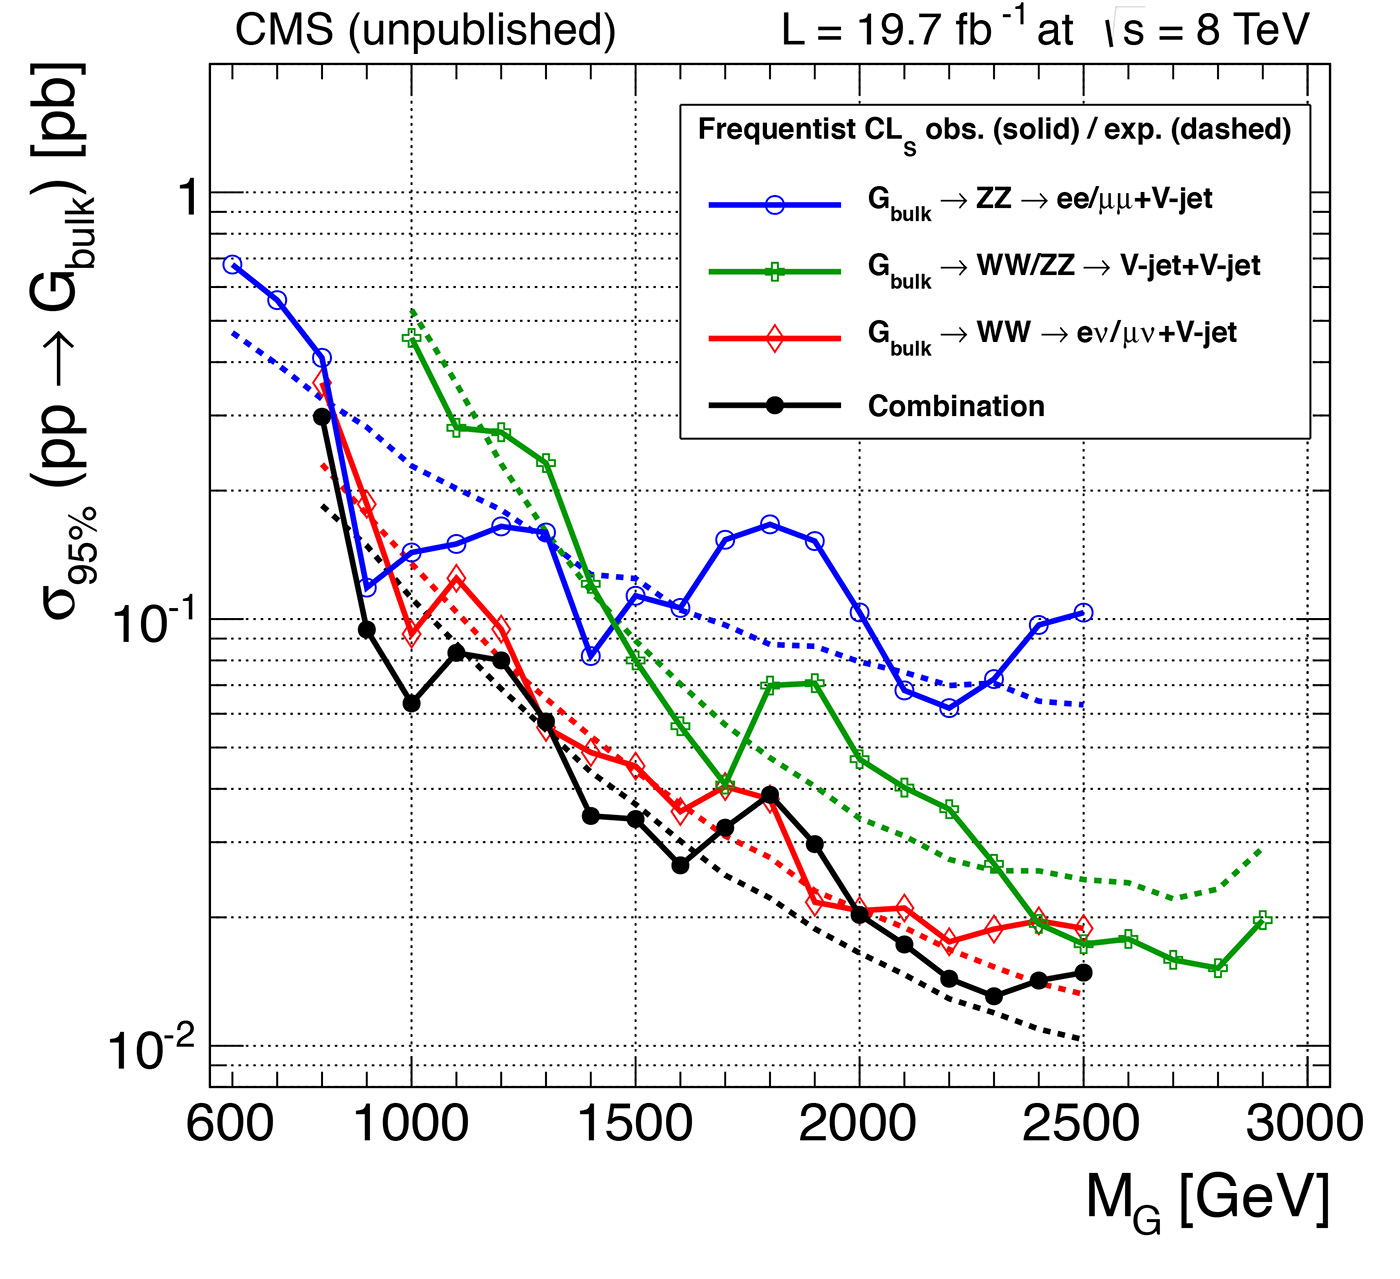
\includegraphics[width=0.6\textwidth]{figures/objects/CMS_comparison-s.jpg}
\caption[Combine limit at Run 1]{Confidence limits on the bulk graviton production cross section obtained by previous CMS analyses.}
\label{2012result}
\end{center}
\end{figure}

%To allow for the full reconstruction of the signal, it is convenient to focus on signatures with no MET. -- work on those has been performed in the group previously \cite{DavidThesis}. 
 Table \ref{branTable} shows all possible branching ratios of the ZZ final state. The leptons plus jet channel (ZZ $\to$ 2$\ell$2q) presents a good balance in between high event yield with a 14\% branching ratio\footnote{This branching ratio refers to decays to the three lepton flavours.} and ease of triggering and selection of the signal events. We chose the bulk graviton model as our benchmark due to its large branching ratio into vector bosons, and particularly on the ZZ channel. Figure \ref{VZchannel} shows the diagram of the signal process, involving the gluon fusion production of the bulk graviton decaying through pair of Z bosons to a $\ell\ell$qq state. The products coming from the decay of a boosted Z boson are expected to be close to each other given the high transverse momentum of the parent. 


\begin{table}[h!]
\begin{center}
\caption[Branching ratios]{Branching ratios of the ZZ decay channel into different final states.}
\label{branTable}
\begin{tabular}{lcr}
\hline
\textbf{Channel} & \phantom{xxx}  &\textbf{Branching ratio} \\ \hline
ZZ $\to$ 4q & \phantom{xxx} & 0.49 \\
ZZ $\to$ 2q2$\nu$ & \phantom{xxx} & 0.28 \\
ZZ $\to$ 2$\ell$2q & \phantom{xxx} & 0.14\\
ZZ $\to$ 2$\ell$2$\nu$ & \phantom{xxx} & 0.04 \\
ZZ $\to$ 4$\nu$ & \phantom{xxx} & 0.04 \\
ZZ $\to$ 4$\ell$ & \phantom{xxx} & 0.01 \\
\hline
\end{tabular}
\end{center}
\end{table}

\begin{figure}[htb!]
\begin{center}
\raisebox{0.25\height}{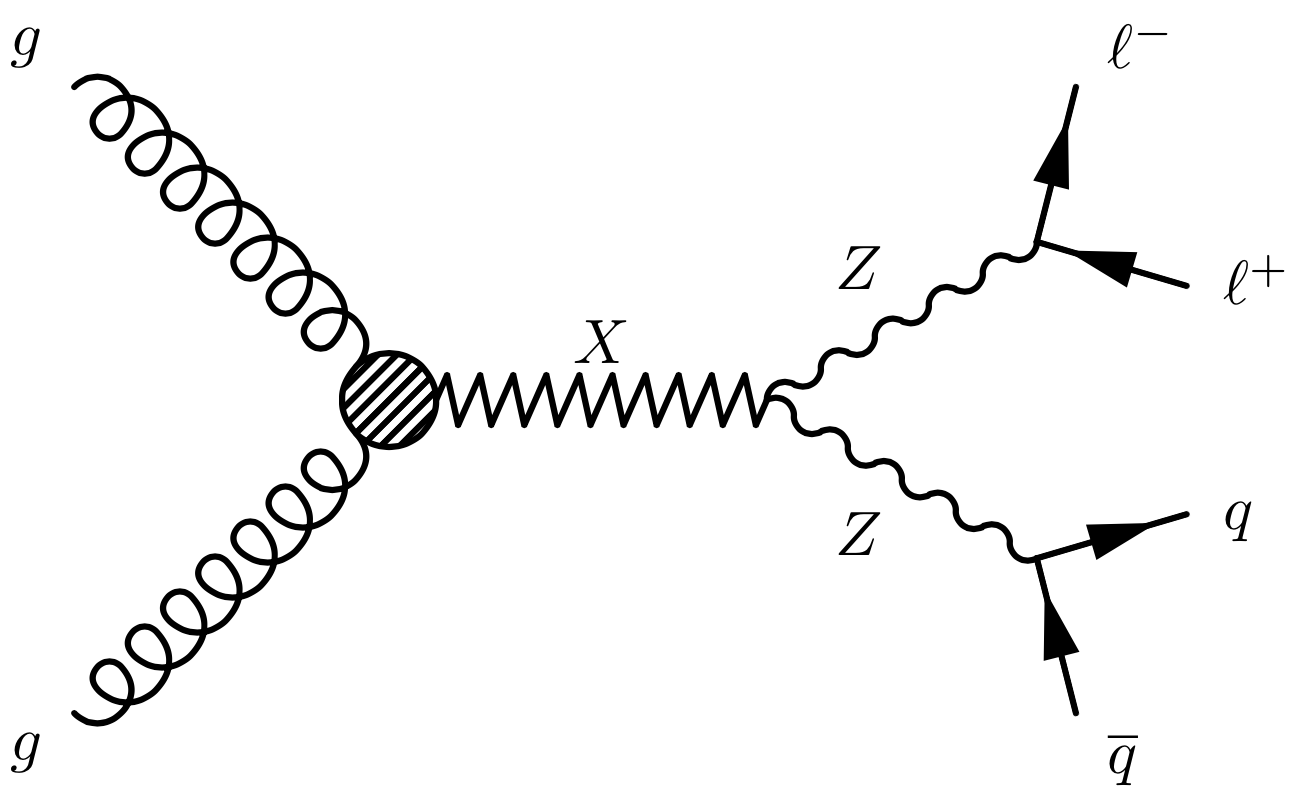
\includegraphics[width=0.45\textwidth]{figures/objects/VZchannel.png}}
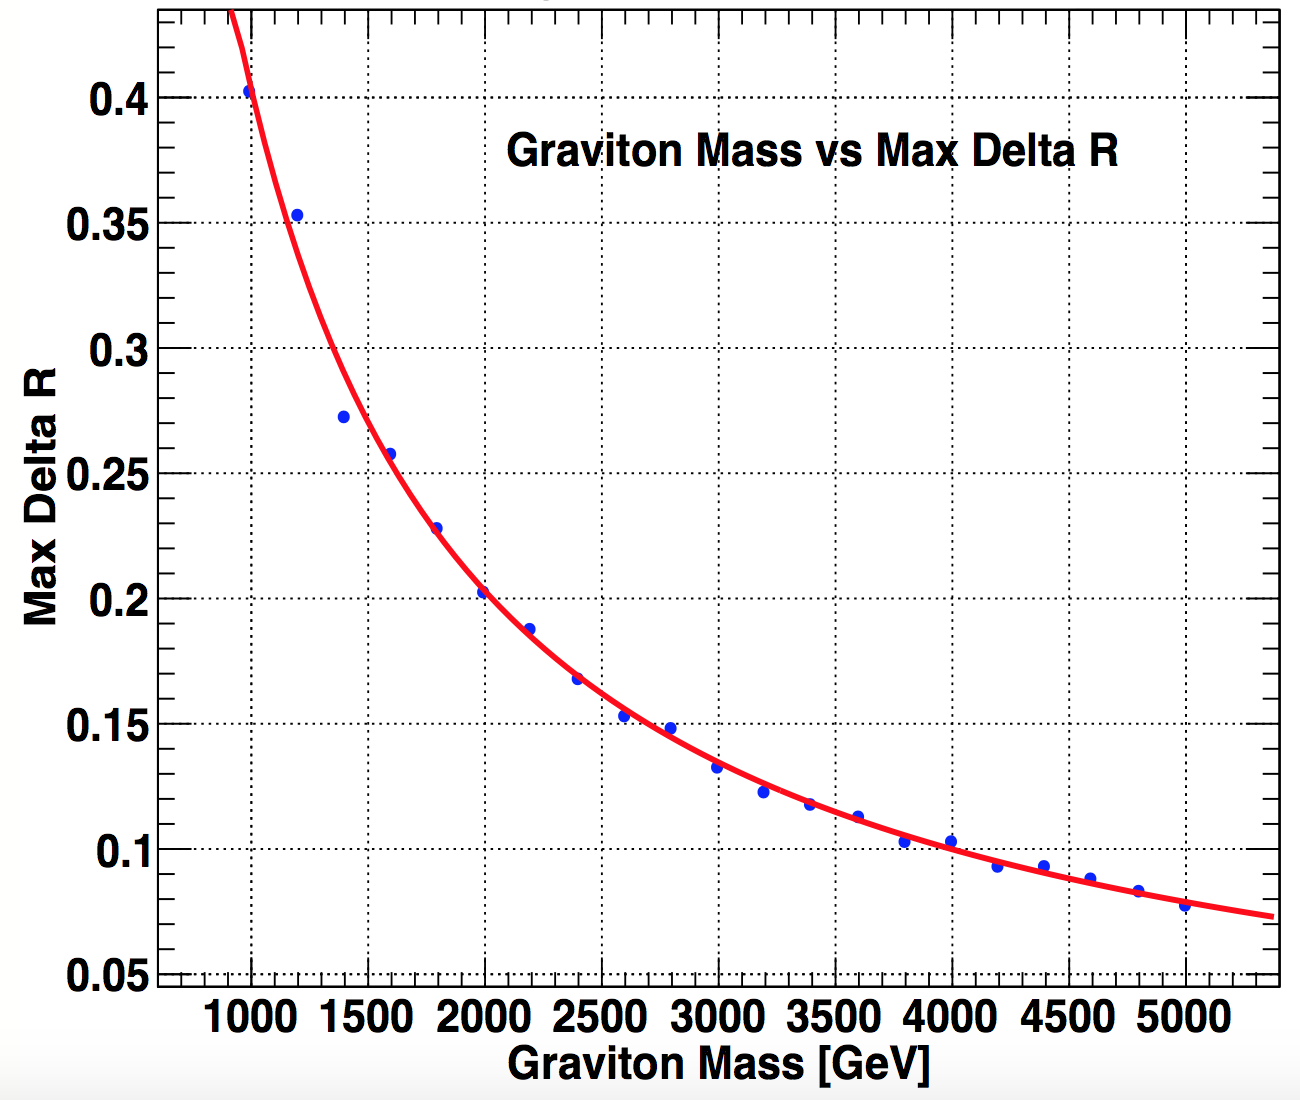
\includegraphics[width=0.50\textwidth]{figures/objects/deltaRvsMass.png}
\caption[Production and decay channel]{Production and decay of a resonance $X$ in the ZZ semi-leptonic channel (left), and separation between the Z boson decay products as function of the graviton mass (right).}
\label{VZchannel}
\end{center}
\end{figure}

The separation between the Z boson decay products, measured in term of $\Delta R = \sqrt{(\Delta\eta)^2 + (\Delta\phi)^2}$, is shown in Fig. \ref{VZchannel} as function of the graviton mass. For high mass of the bulk graviton, the hadronization of two boosted quarks coming from one of the Z's will be reconstructed as a single jet. The pair of leptons that comes from the decay of the other Z boson are also expected to be close to each other. The final state of interest is therefore a dilepton plus a merged jet.

\clearpage
\section{Analysis Strategy}

In order to confront the results obtained in the Run 1, the Run 2 version of the analysis should have used the very same software and analysis framework. However, the different accelerator conditions ($8 \rightarrow 13$ TeV) and the incorporation of a new CMS data format (AOD $\rightarrow$ MiniAOD) forced us to develop original analysis tools, giving rise to the SPRACE analysis framework \cite{spraceFramework}.

%\todo{\large  I did not like this start!!! You must tell more general things in the beginning. Why is important to analyze data in general? How do you compare with theoretical predictions? Pu an overview about you are going to tell us in the chapter. Just after that you mention YOUR particular strategy to attack your problem. } 

The SPRACE framework handles CMS real data in MiniAOD format, as well as data from Monte Carlo simulations. Both real data and simulation need to be split into signal and background. For simulation, the separation of the signal from the background is straightforward because the events are labelled accordingly.

The separation of the signal in real data is a challenging problem that requires dedicated selection criteria in order to enhance the final state, namely, two opposite-sign same-flavour leptons plus one jet. Generally speaking, the analysis strategy follows a series of stages:

\begin{compact_enumerate}
	\item Get data, both real and simulated samples;
	\item Classify into muon and electron channels;
	\item Classify into high purity and low purity categories;
	\item Classify into signal and control regions;
	\item Blind signal region;
	\item Estimate background for each channel, each category, and each region;
	\item Calculate expected limits for each channel and category;
	\item Unblind signal region;
	\item Calculate observed limits for each channel and category;
	\item Combine individual limits. 
\end{compact_enumerate}

The separation between muon and electron channel is a standard choice among CMS analyses. In our case, the muon channel is more competitive than the electron channel providing more sensitivity limits. It is due to the fact that different components of the detector are used in the reconstruction of the objects, translating into different selection criteria and consequently, different efficiencies. 

The split into high purity and low purity categories is another enhancement of the analysis. It takes advantage of the N-subjettiness discriminator introduced in Section \ref{JetSection} to characterize hadronic V jets. By definition, the high purity category contains a larger fraction of signal events than the low purity category. Despite being less efficient, the low purity category slightly improves the sensitivity of the final limit because it allows to retain some signal events in the situation when the expected background approaches to zero. %In our analysis, the expected background approaches to zero for high values of the diboson invariant mass, as will be shown later on.  

The classification into signal and control region intends to reduce the bias in the estimation of the background. In a initial stage of the analysis, the kinematic distributions in the signal region cannot be shown, and only information from the control region is used for background estimation purposes. Only at the end of the analysis the signal region is revealed, and the predictions obtained previously are confronted with the real data.  

In the next section we introduce the selection criteria applied to select signal events and reject background. Basic distributions at generator level, demonstrating properties of the bulk graviton model in contrast to the background processes, are also presented.   

\section{Event Selection}

Semi-leptonic events in the boosted regime, characterized by low $\Delta R$ between the Z boson decay products, can be selected with the set of criteria presented in Table~\ref{tab:cutsummary}. The same selection criteria apply to both real data and simulation, and they are intended to select signal-like events and reject the background. Some justifications for these specific requirements are:

\begin{compact_itemize}
\item The High Level Trigger is based on the presence of a lepton to minimize purely hadronic backgrounds. Since the online reconstruction is optimized for speed instead of accuracy, we chose single lepton triggers to maximize the probability of selecting an event, even though eventually require two reconstructed leptons in the offline analysis.
	
\item Electrons reconstructed in the calorimeter can be faked by QCD jets, requiring a high threshold in the transverse momentum, namely \ptrans $>$ 105 GeV.
	
%\item For muons, RPC detectors localized in the acceptance region $|\eta| < 2.1$ are responsible for the online selection.

\item The offline selection in one of the electrons (muons) at \ptrans larger than 115 GeV (50 GeV), ensures events in the plateau of the trigger turn-on. The selection on the other lepton at \ptrans larger than 20 GeV is a standard CMS threshold applied to particle coming from electroweak processes.

\item The dilepton \ptrans threshold at 170 GeV intends to select Z candidates in the boosted region. The mass window of the dilepton pair includes the nominal mass of the Z boson (91.2 GeV), and is wide enough to ensure that lepton energy/momentum scale effects can be essentially neglected.

\item The remaining offline jet requirements are intended to select V jets, and reject purely hadronic jets. The invariant mass selection is a phase space cut that simply reduces the amount of data have to run over. Since we are interested only in graviton masses above 800 GeV, a diboson invariant mass selection above 600 GeV is safe to apply.
\end{compact_itemize}

The V jet selections were gleaned from the Run 1 analysis. Figure \ref{fig:run1plots} shows that the jet mass does indeed have a peak at the value of the Z boson mass, while the $\tau_2/\tau_1$ ratio shows a clear separation between signal and background. Therefore we define two different classification criteria: one based on the jet substructure
\begin{compact_itemize}
\item High purity: jets with $ \tau_2/\tau_1 < 0.45$;
\item Low purity: jets with $ 0.45 < \tau_2/\tau_1 < 0.75$;
\end{compact_itemize}
and one based on the jet mass
\begin{compact_itemize}
\item Signal region: jets with $ 65 < m_j < 105 $ GeV;
\item Control region: jets with $ 20 < m_j < 65 $ GeV or $ 135 < m_j < 220 $ GeV. 
\end{compact_itemize}

The event selection also includes many requirements on detector status, data quality, object identification, among others. The application of the full event selection on real data is described in Chapter \ref{ch:realdata}.


\begin{figure}[p]
\centering
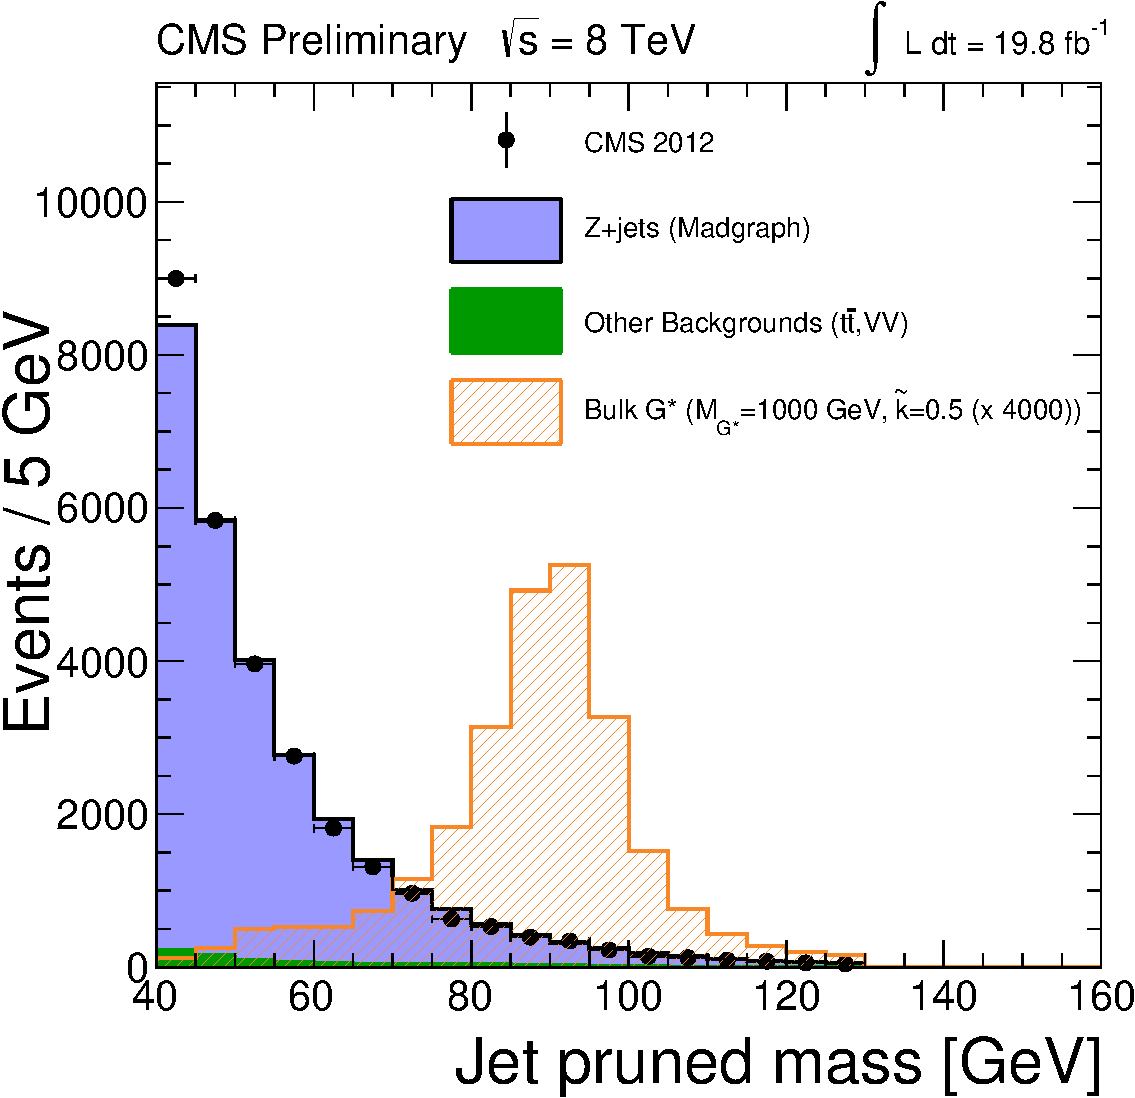
\includegraphics[width=0.6\textwidth]{figures/objects/makePrunedMassPlotForPAS.pdf}\\\vspace{0.5cm}
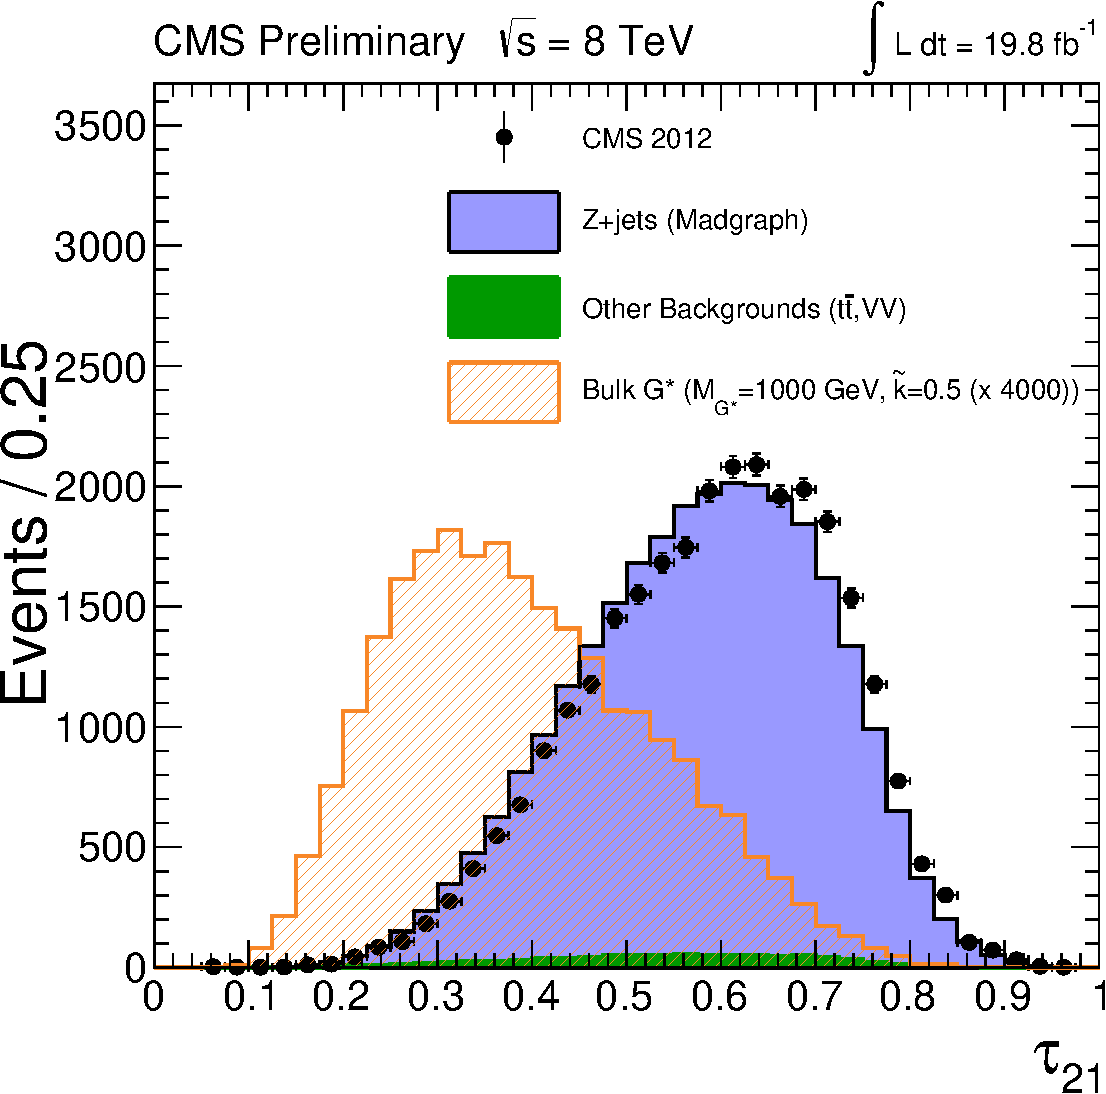
\includegraphics[width=0.6\textwidth]{figures/objects/makeNSubjPlotForPAS.pdf}
\caption[Run 1 analysis]{Jet pruned mass (top) and $\tau_2/\tau_1$ ratio (bottom) taken from the Run 1 analysis \cite{CMS:2013dfa}. The signal region is defined around the peak in the jet mass distribution. The high purity category includes low values of $\tau_{21}$, where the signal is concentrated.}
\label{fig:run1plots}
\end{figure}


\begin{landscape}
\begin{table}[p]
%\footnotesize
%\scriptsize
\begin{center}
\caption{Summary of the event selection.}
\label{tab:cutsummary}
\begin{tabular}{lcc}
\hline
\multicolumn{1}{c}{\textbf{Selection}} & \textbf{Value} \T& \textbf{Comments}\\
\hline
\multicolumn{1}{c}{High Level Trigger \T}\\
\cline{1-1}
Electron channel  & \ptrans $> 105$ GeV  \T& \\
Muon channel      & \ptrans $> 45$ GeV and $|\eta|<2.1$  \T& \\
\hline
\multicolumn{1}{c}{Electrons\T}\\
\cline{1-1}
Electron ID   & Loose working point  \T& \\
Isolation       & Particle flow isolation  \T& \\
Acceptance  & \ptrans$ > 115 $ GeV,  $|\eta|<2.5$    \T &  leading or second electron\\
                     & \ptrans$ > 20 $ GeV,  $|\eta|<2.5$    \T  &  remaining electron\\
\hline
\multicolumn{1}{c}{Muons\T}\\
\cline{1-1}
Muon ID       & High \ptrans or tracker high \ptrans            \T   & At least 1 high \ptrans \\
Isolation       & Tracker isolation with inner track removal   \T   & \\
Acceptance  & \ptrans$ > 50 $ GeV,  $|\eta|<2.1$            \T  &  leading or second muon\\
                     & \ptrans$ > 20 $ GeV,  $|\eta|<2.4$           \T  &  remaining muon\\
\hline
\multicolumn{1}{c}{Dilepton selection\T}\\
\cline{1-1}
Leptonic Z    &  \ptrans$ > 170 $ GeV                   \T& \\
                     &  $70<M_{\ell\ell}<110$ GeV     \T& \\
\hline
\multicolumn{1}{c}{AK8 Jets \T}\\
\cline{1-1}
Jet ID           &  Loose working point               \T  & cleaning w.r.t. \\
Acceptance  &  \ptrans$ >200$ GeV, $|\eta|<2.4$ \T & good leptons  \\
Jet mass (signal region)                & $ 65 < m_j < 105 $ GeV \T&  \\
Jet mass (low mass control region)       & $ 20 < m_j < 65 $ GeV \T& \\
Jet mass (high mass control region)     & $ 135 < m_j < 220 $ GeV \T& \\
N-subjettiness (low purity)             & $ 0.45 < \tau_2/\tau_1 < 0.75 $  \T& \\
N-subjettiness (high purity)            & $ \tau_2/\tau_1 < 0.45$  \T& \\
\hline
\multicolumn{1}{c}{Diboson candidate \T}\\
\cline{1-1}
Invariant mass & $M_{\rm VZ}>600$ GeV        \T& \\
\hline						       
\end{tabular}
\end{center}
\end{table}
\end{landscape}

\clearpage
\section{Simulated Samples}

To optimize and test our selection, we use a set of simulated background and signal samples. For the final state of choice, the standard model processes that constitute the relevant background are Z+jets, diboson (WW + WZ + ZZ), and $t\bar{t}$. One advantage of the double lepton channel adopted in this search is the absence of QCD backgrounds due to the fact that leptons are not subject to strong interactions. 

For the description of the Z+jets background, a set of samples were generated with the {\sc madgraph} event generator~\cite{Alwall:2014hca}. The samples are binned according to the variable HT, which is the sum of the transverse energies of partons at matrix-element level. The split in HT bins reduces the computational time specially for high values of this variable, where a re-weighting factor is used to increase the number of available events in the sample. In this way, we can explore this background for high values of the reconstructed diboson invariant mass, since it is correlated with HT. Samples of $t\bar{t}$ and SM diboson production are generated using {\sc powheg} 2~\cite{Nason:2004,Frixione:2007,Alioli:2008} and {\sc pythia} 8~\cite{PYTHIA6, PYTHIA8}, respectively.

Bulk graviton signal events are generated with {\sc madgraph} setting $k/M_{Pl} = 0.5$; 
under this condition, the natural width of the resonance is much smaller than the experimental resolution. Working with narrow resonances is convenient because we can easily extrapolate to lower values of the bulk graviton model parameter, since that would minimally affect the shape of the diboson invariant mass distribution.
Parton showering and hadronization processes are simulated by interfacing the event generators to {\sc pythia} 8 with the CUETP8M1~\cite{Skands:2014pea} tune.
The NNPDF 3.0 parton distribution functions (PDF)~\cite{Ball2015} are used to model the momentum distribution of the colliding partons inside the protons. For both signal and background Monte Carlo (MC) samples, events are simulated using a {\sc Geant4}-based model~\cite{GEANT4} of the CMS detector and processed using the same reconstruction algorithms as for real data. 

Supplementary minimum bias interactions are added to the generated events in order to match the additional particle production observed in real data from the large number of pileup interactions. In this context, minimum bias events account the inelastic non-diffrative part of the total cross section. Assuming a proton-proton total cross section of $\sigma_{tot} \sim 100$~mb, the minimum bias component would be close to $2/3\,\sigma_{tot} \sim 70$~mb \cite{CMS:2016ael}.

%The additional particle production observed in real data due to the large number of pileup interactions is also simulated in the samples. In order to save computing time, instead of simulating the pileup for each individual event we employ a special library of events with pre-simulated interactions. The library contains minimum bias \footnote{In this context, minimum bias means the eikonalized description of hard QCD processes available in {\sc pythia} 8, intended to represent the almost totality of pileup events at the LHC.} events that simulate the pileup of $N$ events over the event of interest, we add the DIGIs of $N$ events from that set to the DIGIs of the event of interest. The total set of DIGIs is then passed onwards to the further steps of reconstruction and analysis.

%\begin{landscape}
\begin{table}[p]
%\scriptsize
\centering
\caption[Description of the simulated samples.]{Description of the simulated samples. Z+jets background were generated with the {\sc madgraph}. $t\bar{t}$ and SM diboson production are generated using {\sc powheg} 2 and {\sc pythia} 8, respectively. Bulk graviton signal events are generated with {\sc madgraph} setting $k/M_{Pl} = 0.5$. Detector effects are simulated using a {\sc Geant4}-based model.}
\begin{tabular}{lrrr}
\textbf{Sample name} & \textbf{Cross section[pb]} & \textbf{N\textsubscript{events}} \\
\hline
DYJetsToLL\tus{}M-50\tus{}HT-100to200 &     147.40 x 1.23	& 2655294	 \\
DYJetsToLL\tus{}M-50\tus{}HT-200to400 &	40.99  x 1.23	&  962195 	 \\
DYJetsToLL\tus{}M-50\tus{}HT-400to600 &	5.678  x 1.23	& 1069003	 \\
DYJetsToLL\tus{}M-50\tus{}HT-600toInf  &	2.198  x 1.23	&  1031103         \\
\hline
WW                &  118.7 & 988418 \\
WZ                &    66.1 & 1000000 \\
ZZ                &   15.4   & 985600 \\
\hline
TT &    831.76  & 196937036 \\

\hline
%/BulkGravToZZToZlepZhad\tus{}narrow\tus{}M-600\tus{}13TeV-madgraph  & 226E-3 & 50000 \\
BulkGravToZZToZlepZhad\tus{}narrow\tus{}M-800   & 41.7E-3 & 50000 \\	 
BulkGravToZZToZlepZhad\tus{}narrow\tus{}M-1000 & 11.2E-3 & 50000 \\	 
BulkGravToZZToZlepZhad\tus{}narrow\tus{}M-1200 & 3.74E-3 & 50000 \\
BulkGravToZZToZlepZhad\tus{}narrow\tus{}M-1400 & 1.44E-3 & 49200 \\
BulkGravToZZToZlepZhad\tus{}narrow\tus{}M-1600 & 0.92E-3 & 50000 \\
BulkGravToZZToZlepZhad\tus{}narrow\tus{}M-1800 & 0.76E-3 & 50000 \\
BulkGravToZZToZlepZhad\tus{}narrow\tus{}M-2000 & 0.135E-3 & 48400 \\
BulkGravToZZToZlepZhad\tus{}narrow\tus{}M-2500 & 0.070E-3 & 50000 \\
%/BulkGravToZZToZlepZhad\tus{}narrow\tus{}M-3000\tus{}13TeV-madgraph & 0.006E-3 & 50000 \\
\hline
\end{tabular}
\label{tab:VZSamples}
\end{table}
%\end{landscape}

\section{Signal Characterization}
As we mentioned earlier, the presence of two leptons in the final state reduces considerably the background rate. Moreover, the kinematics of leptons coming from a boosted Z boson, typical signature of signal events, is different than the distribution of regular Z bosons produced by background processes. Figure \ref{fig:signalid} shows a selection of generator level distributions for both signal and background. It can be seen that for signal events both the Z boson and the daughter leptons have, in general, much harder \ptrans than in background events.

\begin{figure}[p]
\centering
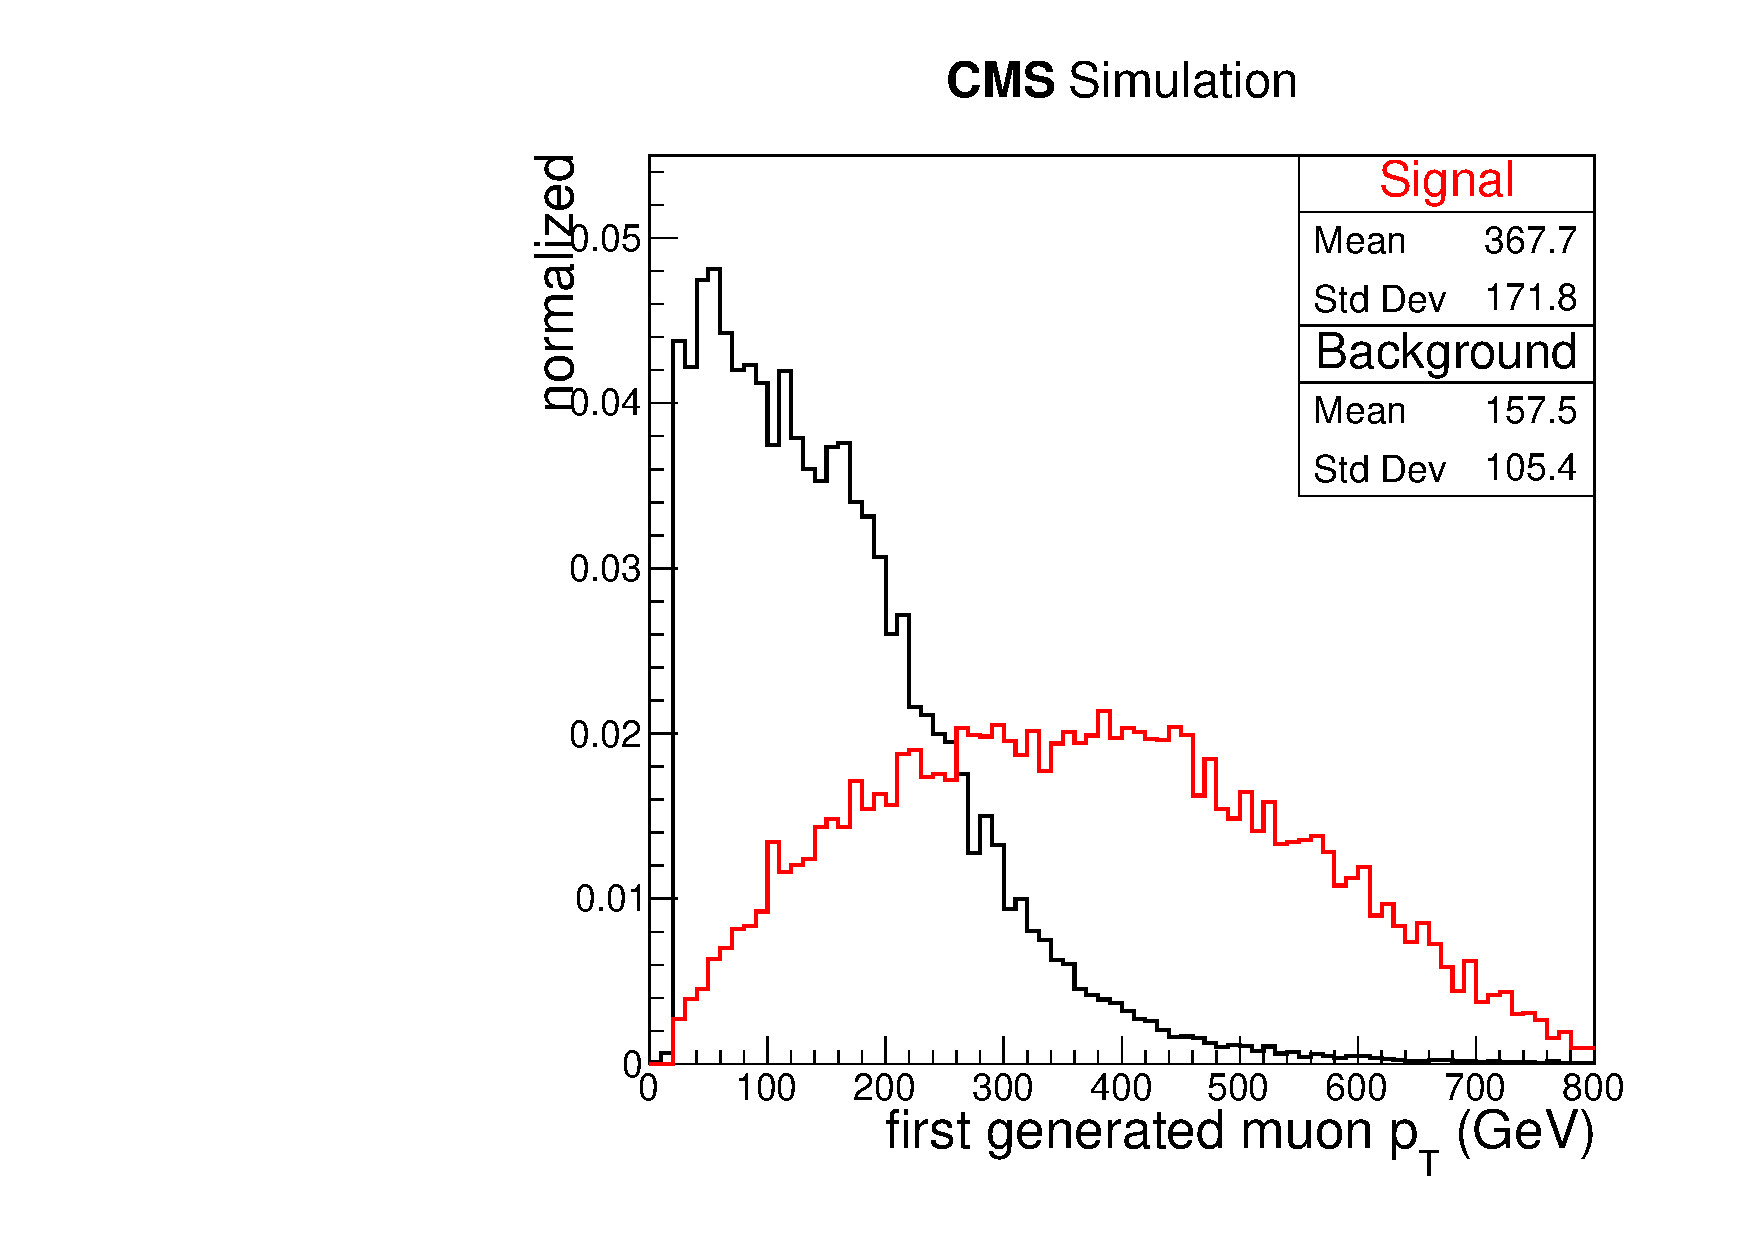
\includegraphics[width=0.48\textwidth]{figures/objects/genlep1ptMNP.pdf}
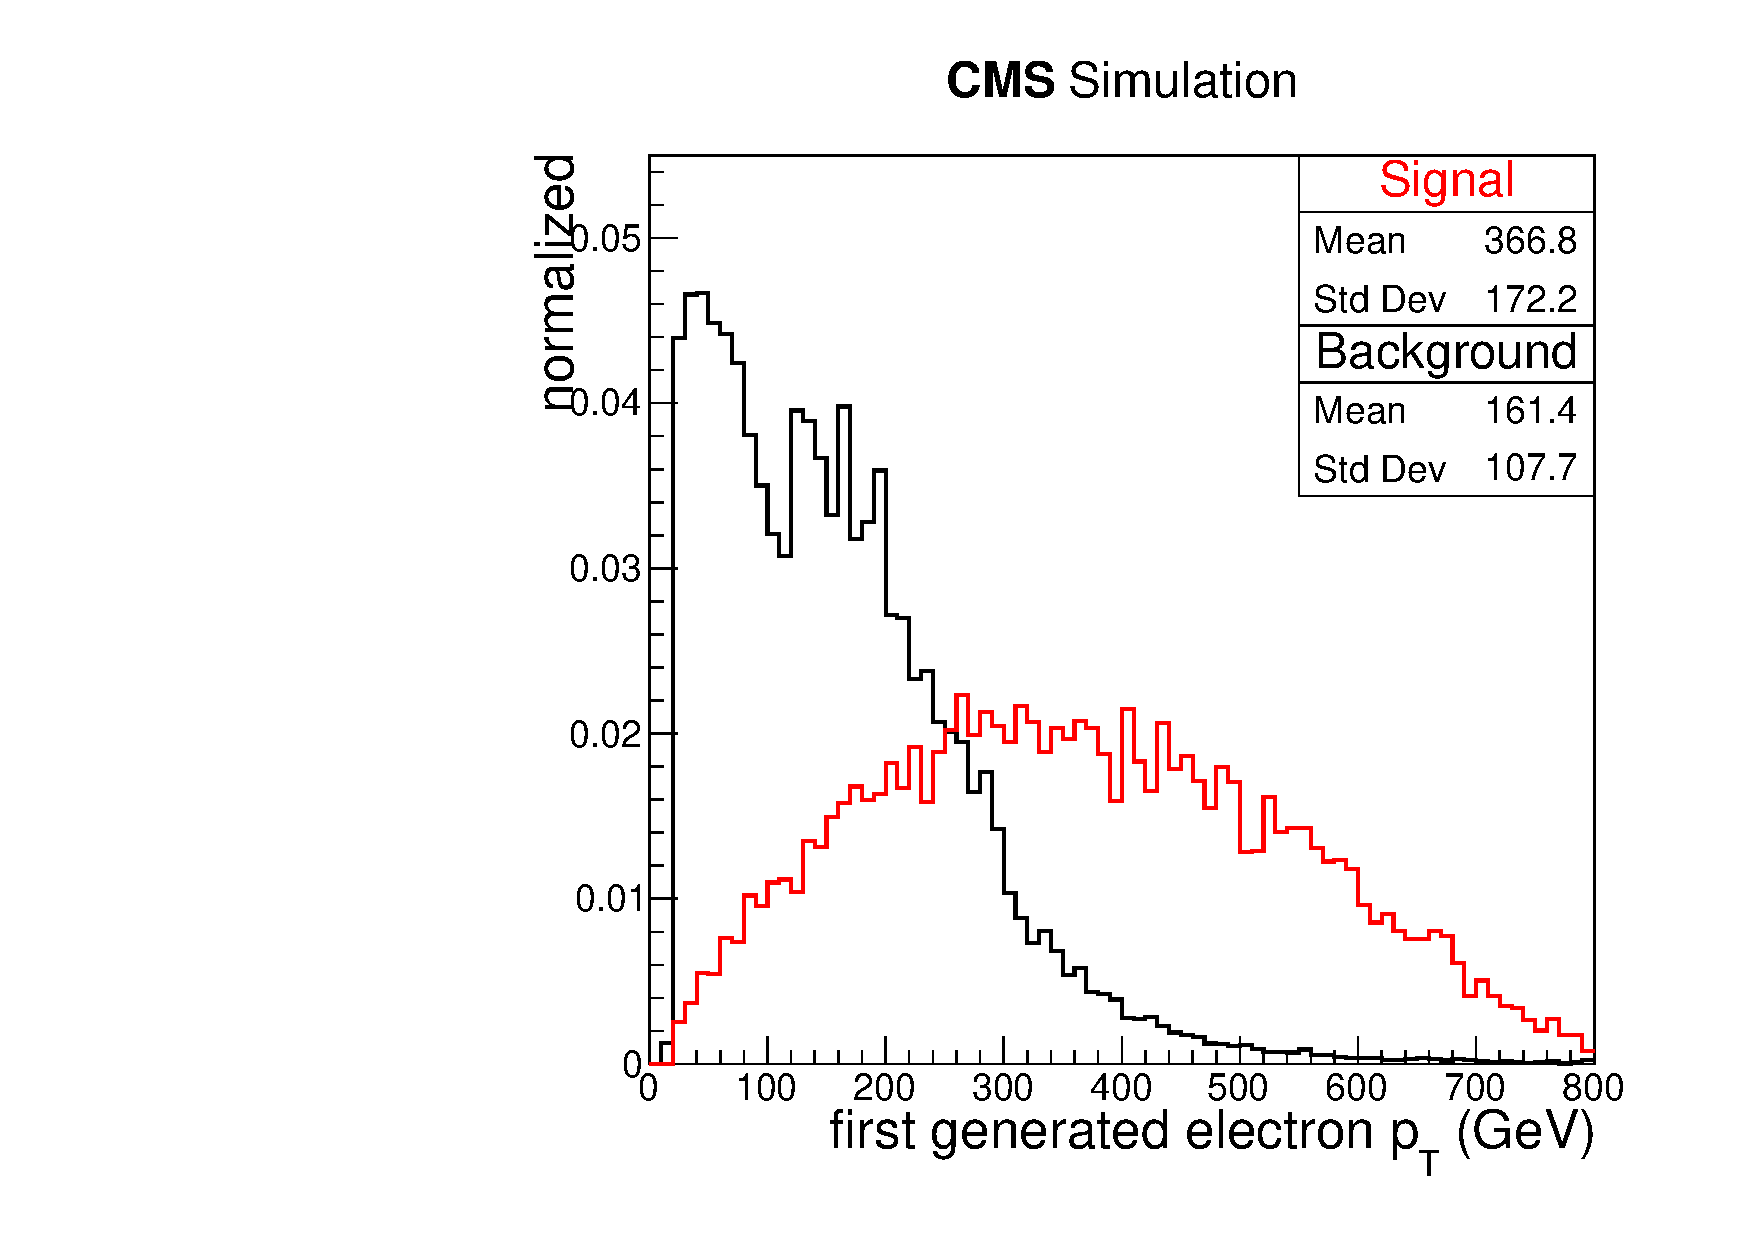
\includegraphics[width=0.48\textwidth]{figures/objects/genlep1ptENP.pdf}\\
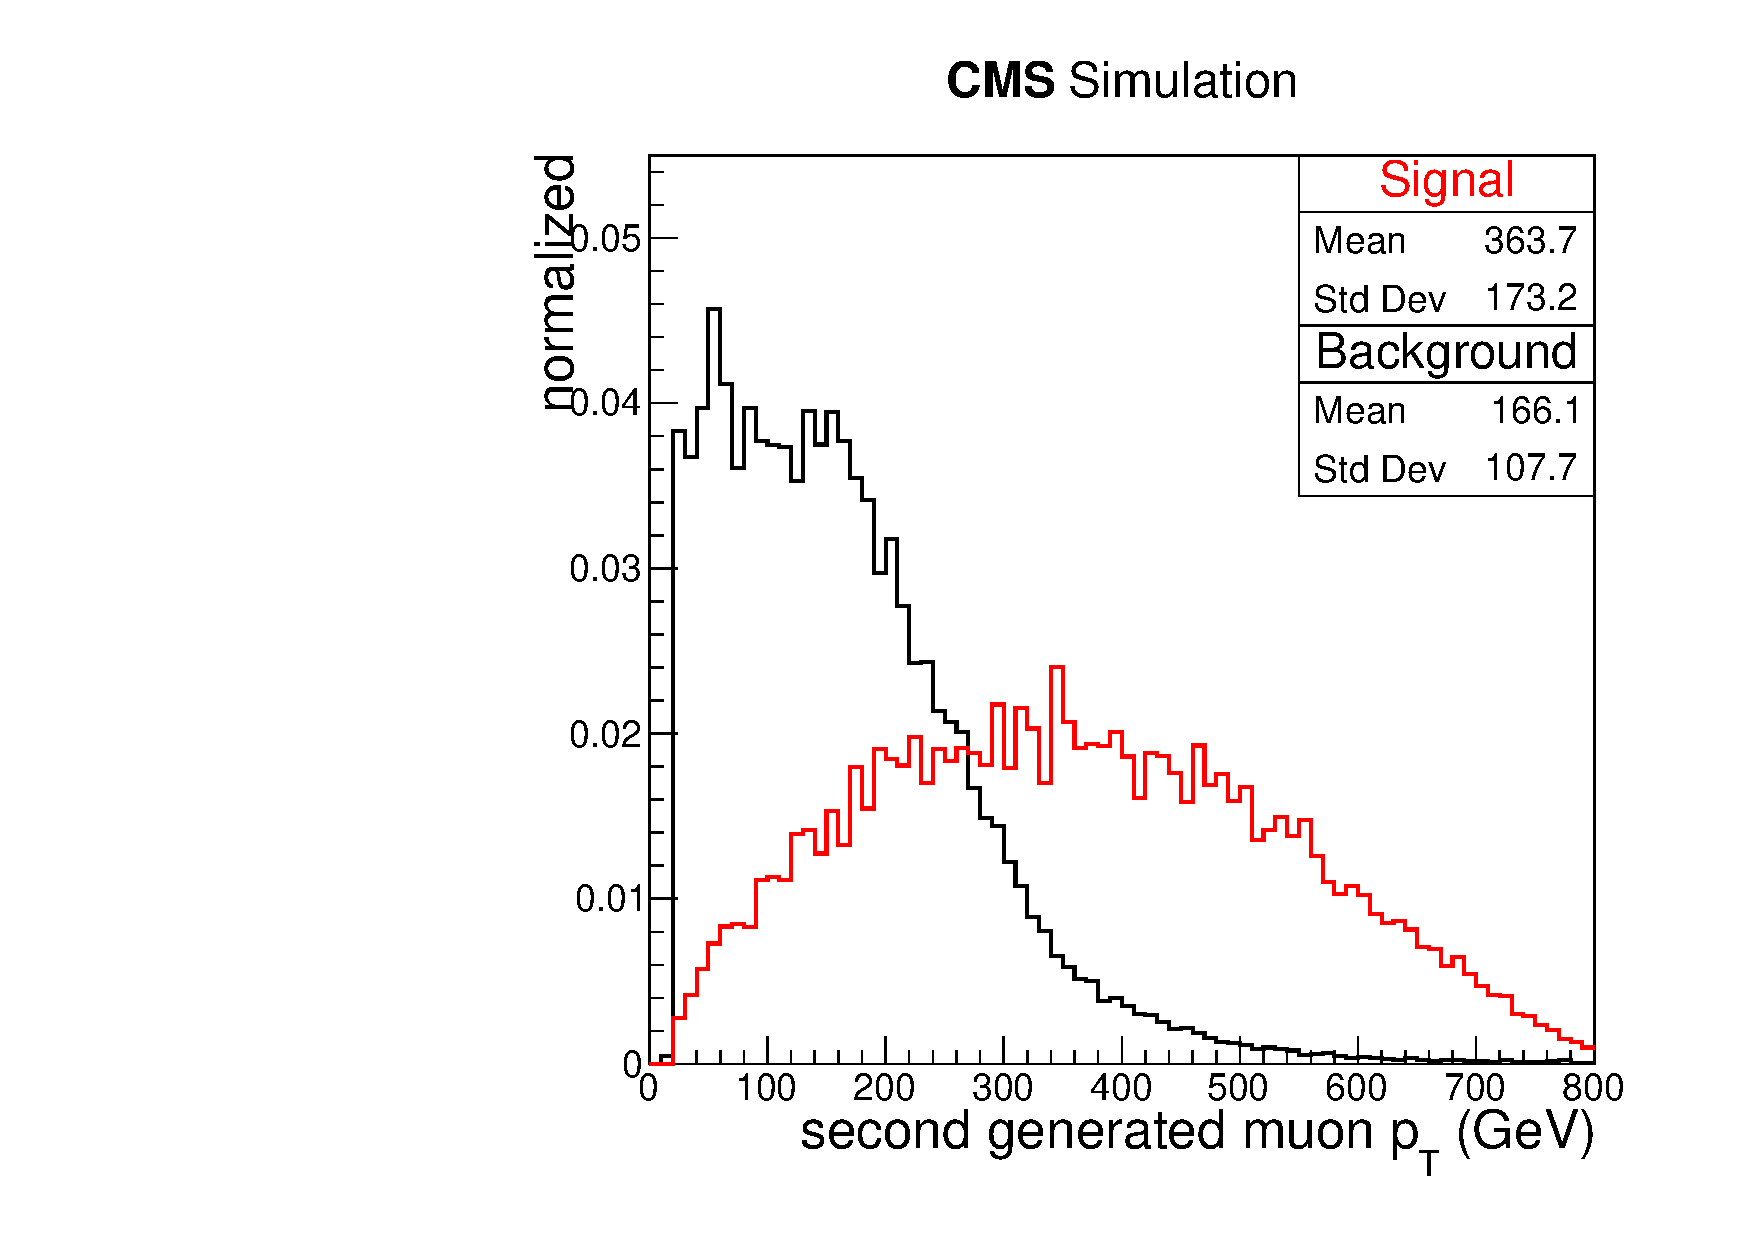
\includegraphics[width=0.48\textwidth]{figures/objects/genlep2ptMNP.pdf}
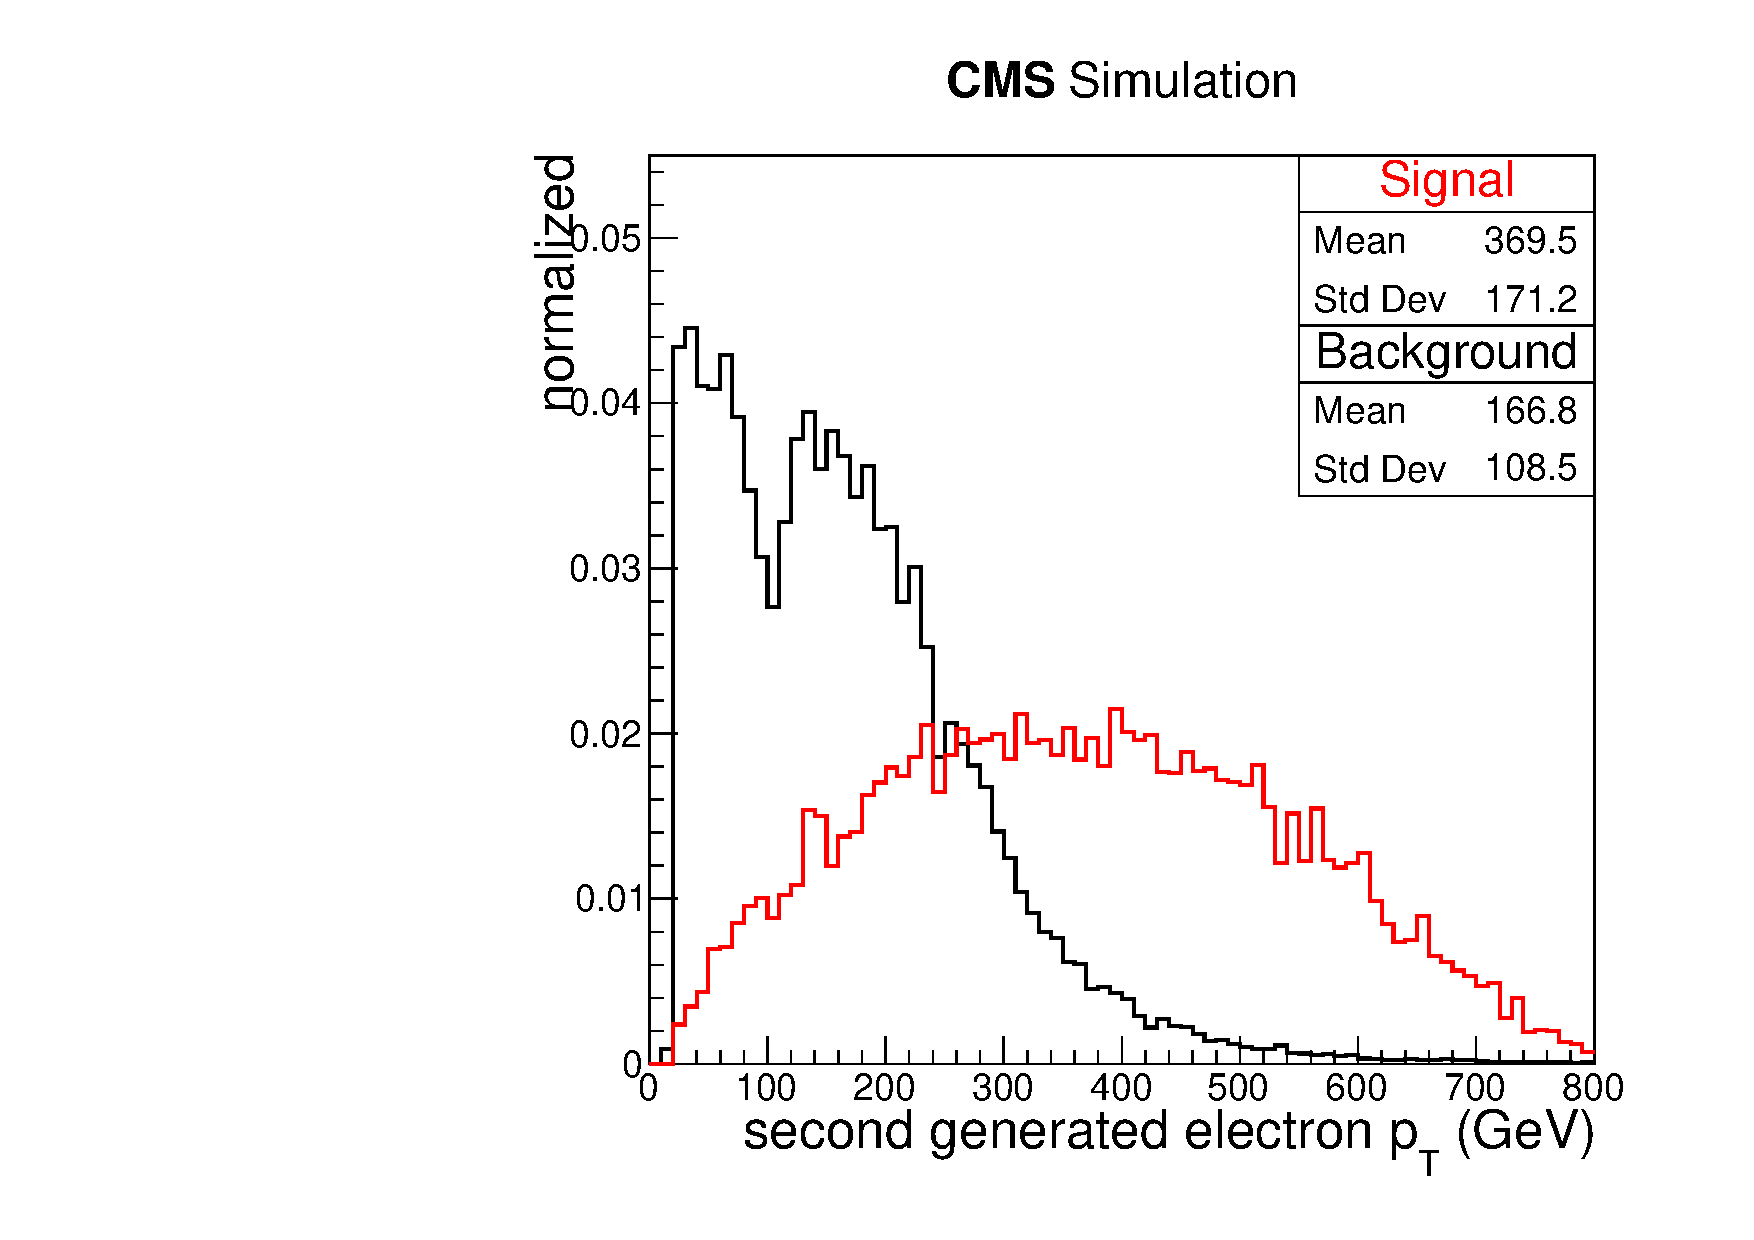
\includegraphics[width=0.48\textwidth]{figures/objects/genlep2ptENP.pdf}\\
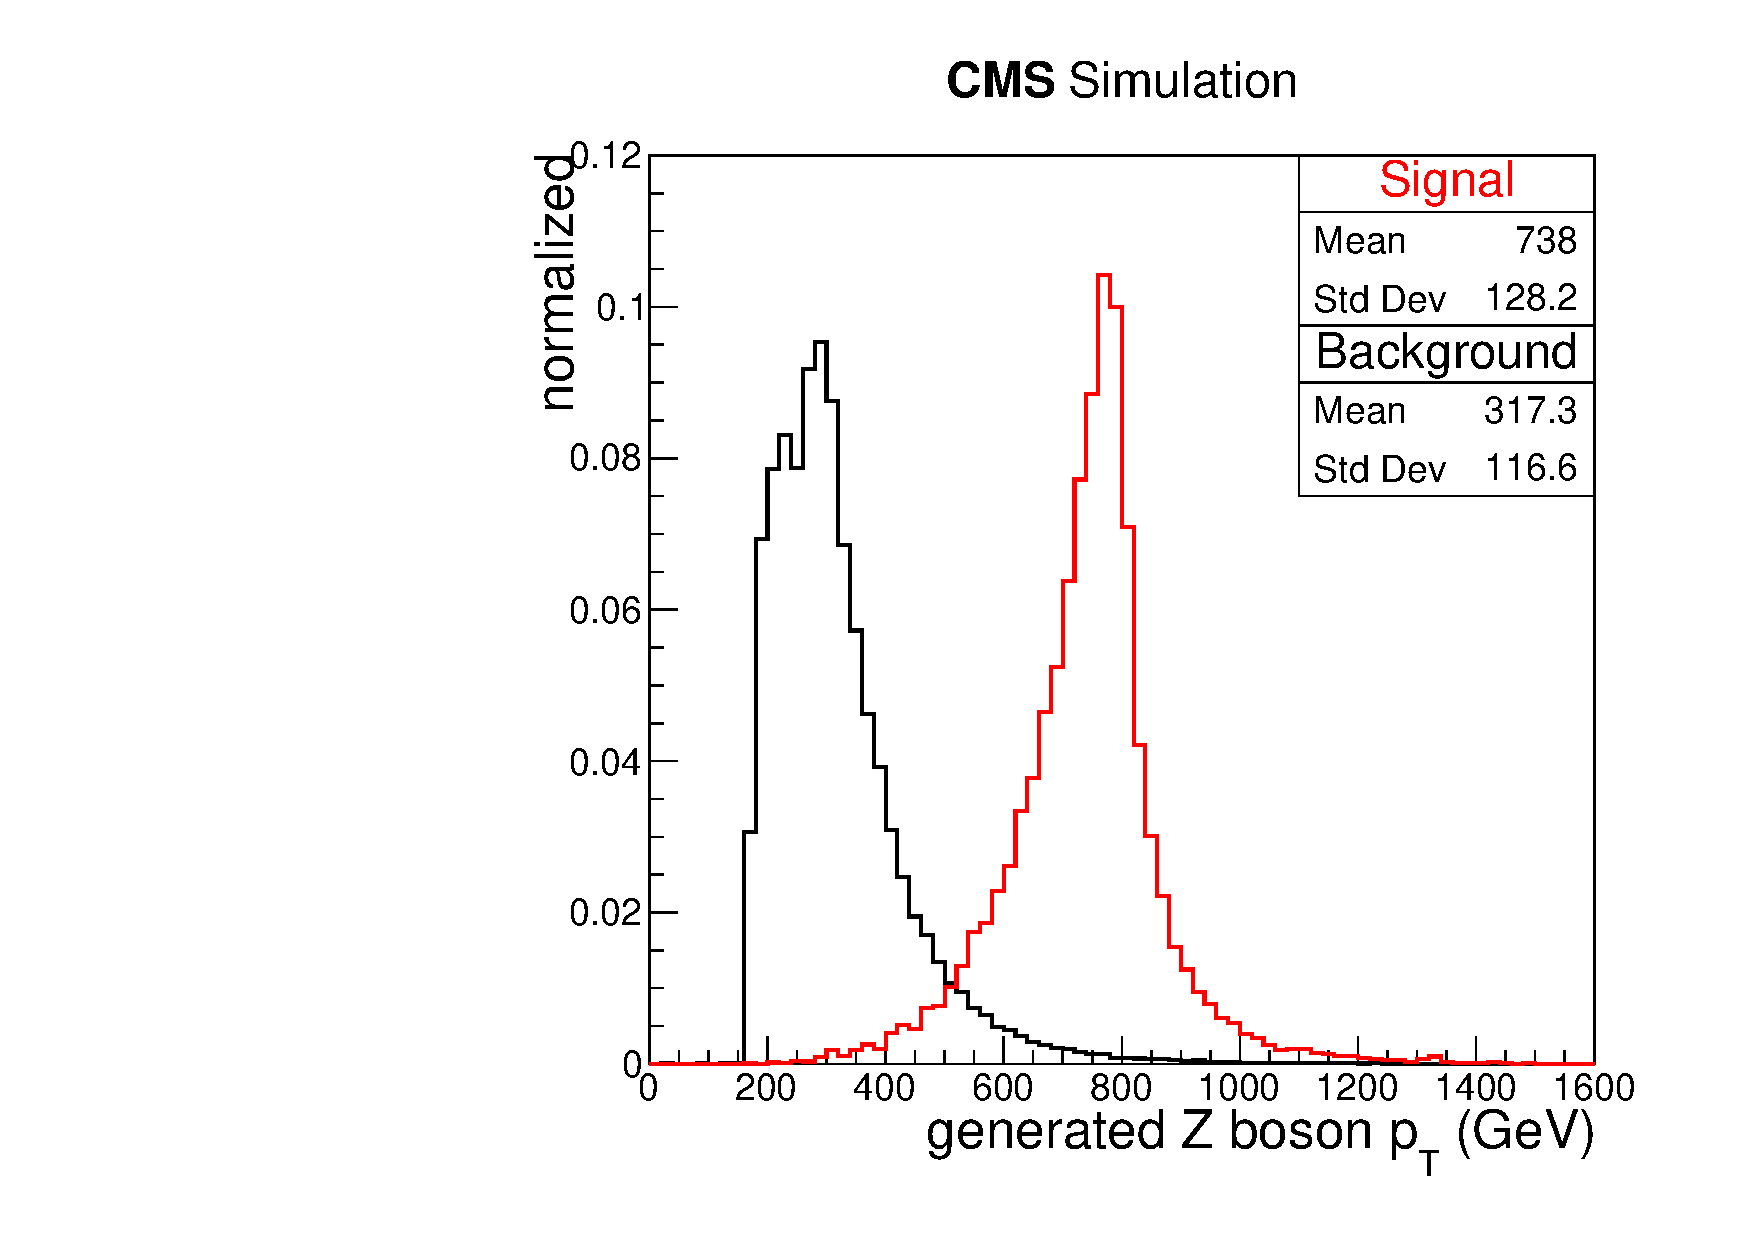
\includegraphics[width=0.48\textwidth]{figures/objects/genZptMNP.pdf}
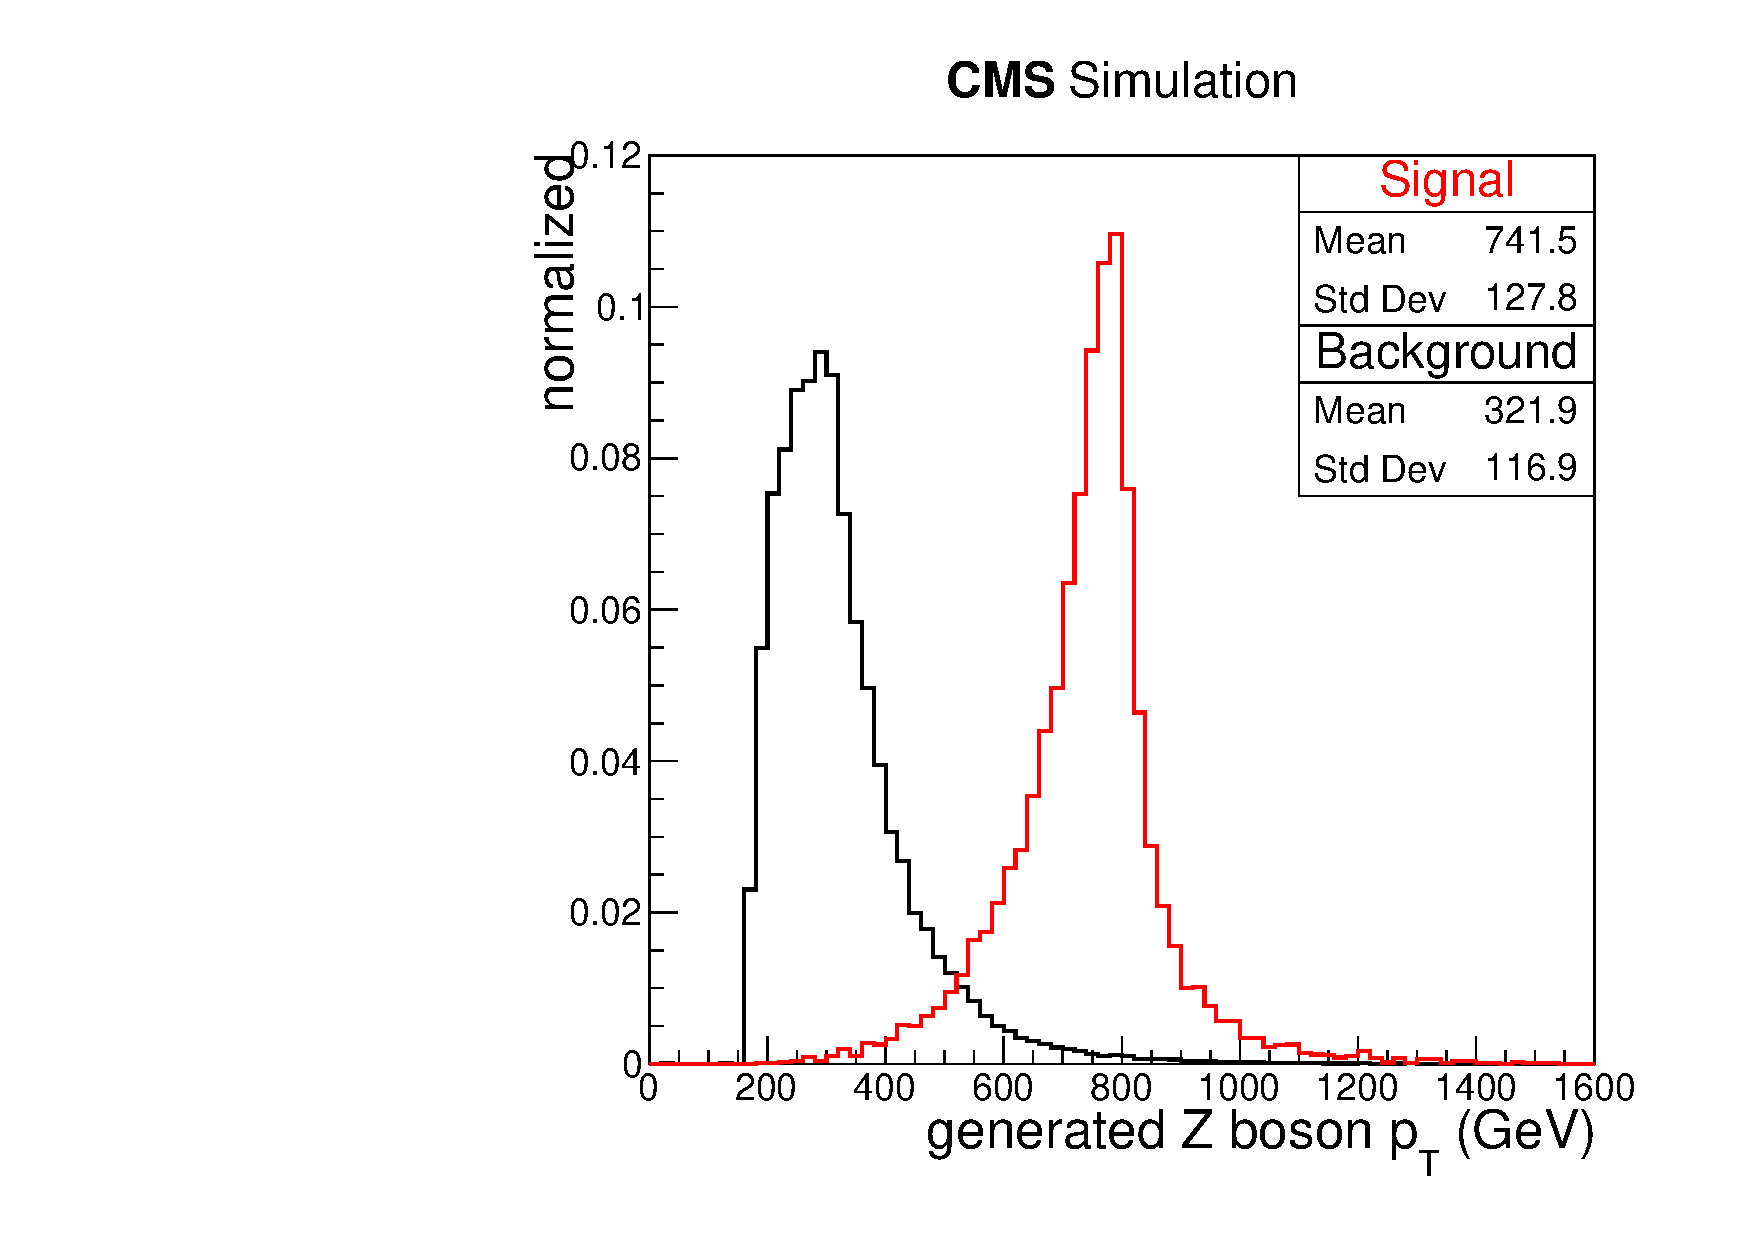
\includegraphics[width=0.48\textwidth]{figures/objects/genZptENP.pdf}
\caption[Signal characterization]{Z boson transverse momentum at generator level and leptons kinematics in the muon (left) and electron (right) channels. The signal corresponds to a bulk graviton of mass 1.6 GeV; the background corresponds to standard model processes described in Table \ref{tab:VZSamples}. All distributions are normalized to unity.}
\label{fig:signalid}
\end{figure}

For modeling the signal invariant mass we use a probability density function consisting of a gaussian peak and a power-law in both tails ---~double crystal ball~--- defined below:
\begin{eqnarray*}
f(x;\alpha_1,\alpha_2,n_1,n_2,\bar x,\sigma) =& \exp(- \frac{t^2}{2}), & \mbox{for } t > -\alpha_1 \mbox{  and  } t<\alpha_2 \\
=& A_1 \cdot (B_1 - t)^{-n_1}, & \mbox{for } t \leq -\alpha_1 \\
=& A_2 \cdot (B_2 + t)^{-n_2}, & \mbox{for } t \geq \alpha_2
\end{eqnarray*}
where $t = \dfrac{x - \bar x}{\sigma}$ and
\begin{eqnarray*}
A_1 &= \left(\frac{n_1}{\left| \alpha_1 \right|}\right)^{n_1} \cdot \exp\left(- \frac {\alpha_1 ^2}{2}\right) \quad , \quad
B_1 = \frac{n_1}{\left| \alpha_1 \right|}  - \left| \alpha_1 \right|\,,\\
A_2 &= \left(\frac{n_2}{\left| \alpha_2 \right|}\right)^{n_2} \cdot \exp\left(- \frac {\alpha_2 ^2}{2}\right) \quad , \quad
B_2 = \frac{n_2}{\left| \alpha_2 \right|}  - \left| \alpha_2 \right|\,.
\end{eqnarray*}

An interpolation procedure is performed to simulate intermediate mass points in order to search for narrow resonances over the continuous background by steps of 100 GeV, starting at 0.8 TeV up to 2.5 TeV. The signal shapes obtained after the interpolation procedure are shown in Fig. \ref{sigShapes}. At generator level the signal invariant mass would look like a narrow delta function and the width of the double crystal ball resembles the detector resolution; therefore, for higher values of invariant mass the detector resolution is systematically worse. 

The sensitivity of the analysis to the presence of a bulk graviton signal directly depends on the selection efficiency, and in turn, the efficiency depends on the channel and category under consideration. As shown in Fig. \ref{selectionEff_VZ}, the selection efficiency of the muon channel is higher than the electron channel, and the high purity category outperforms the low purity category. 

\begin{figure}[p]
\begin{center}
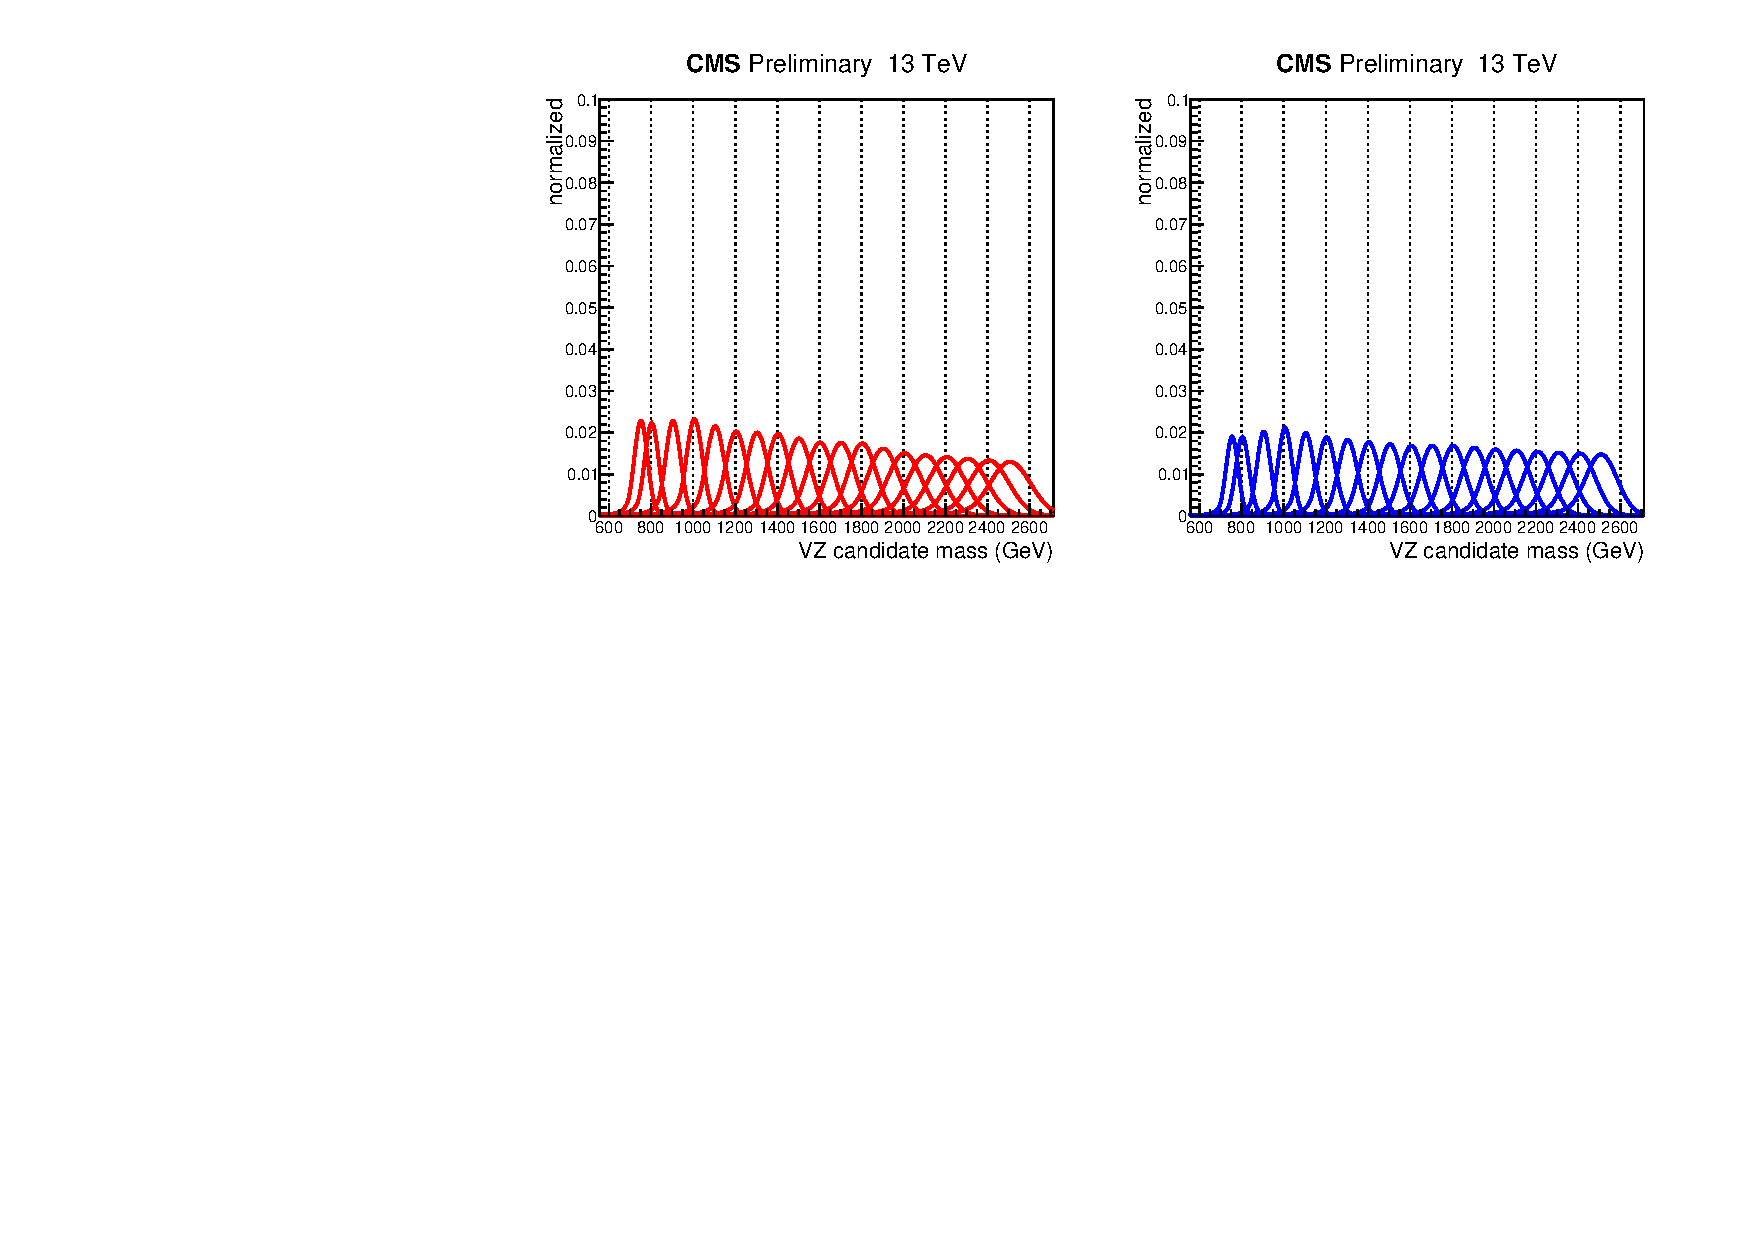
\includegraphics[scale=0.80]{figures/fits/sigShapeLP.pdf}\\
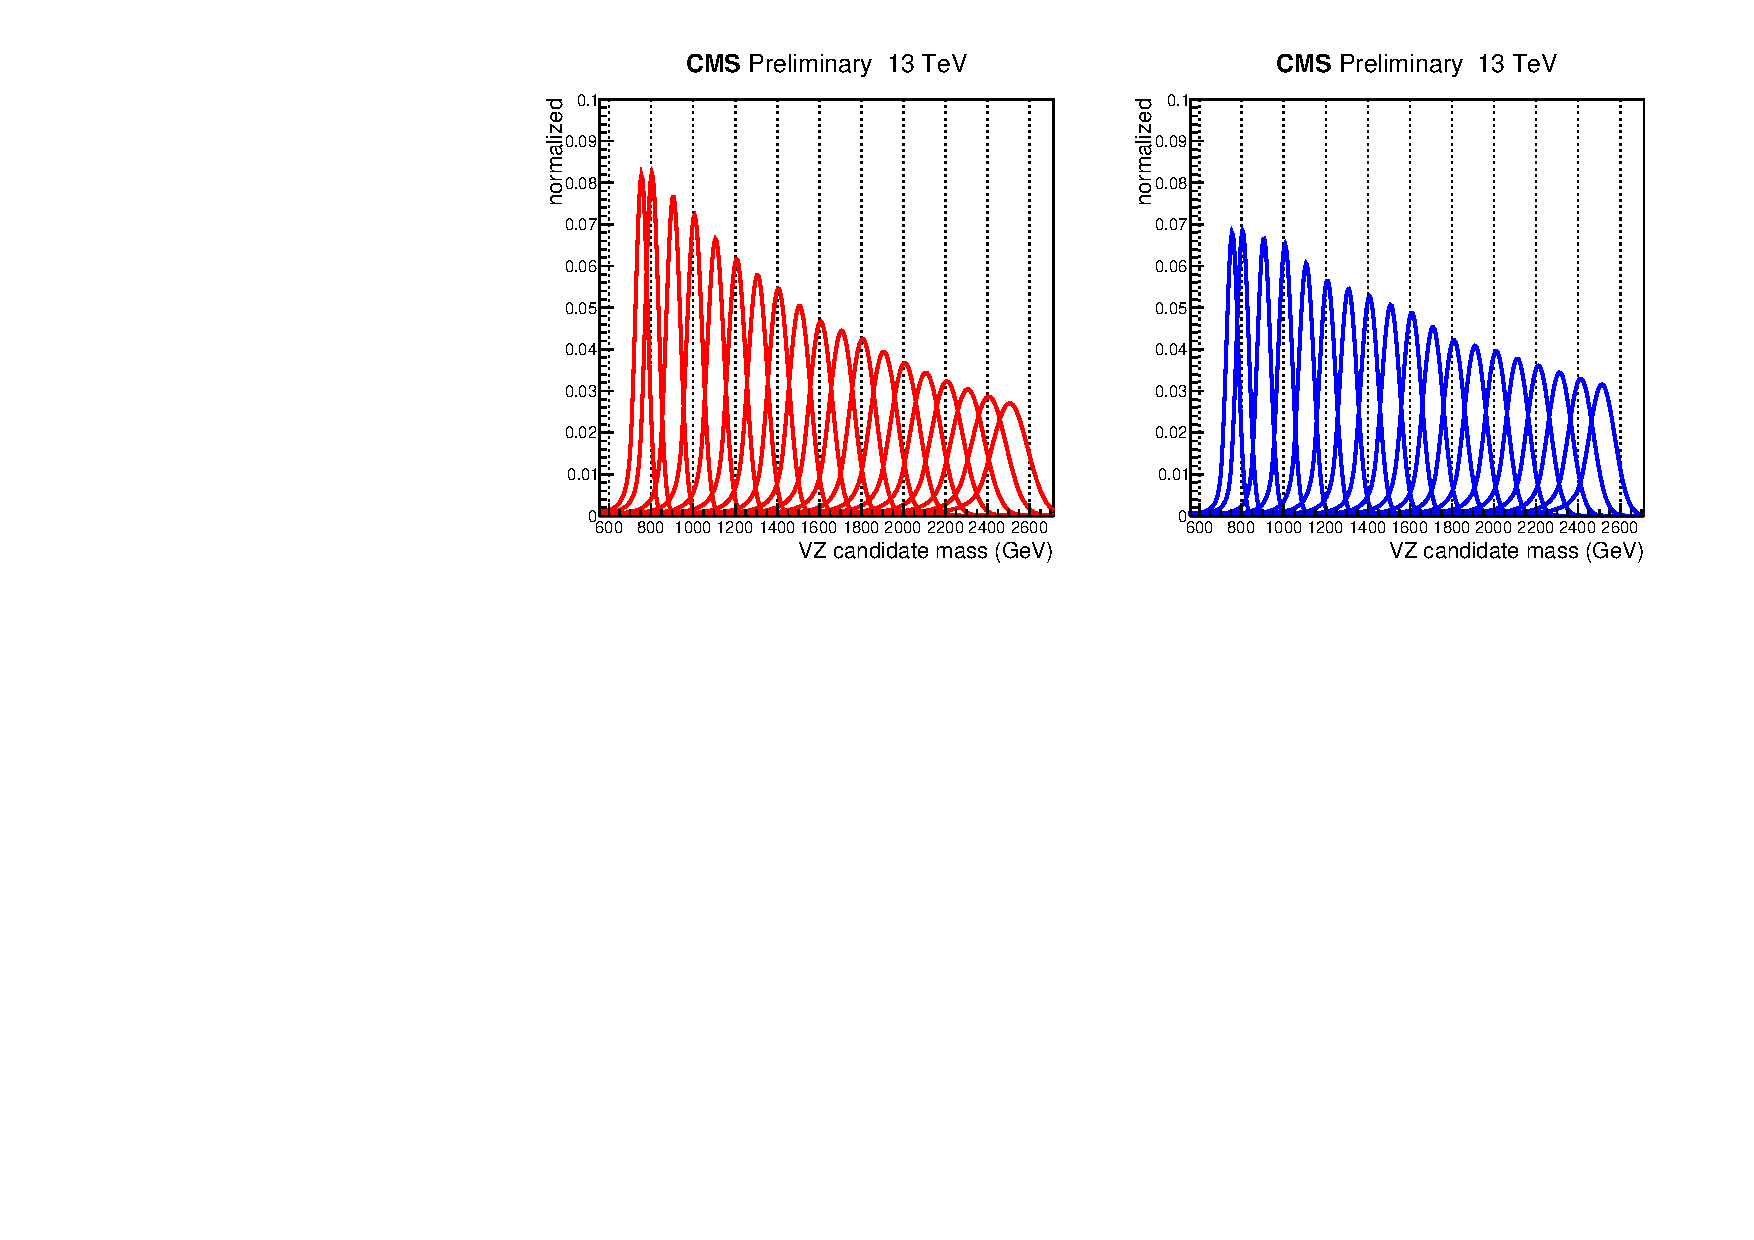
\includegraphics[scale=0.80]{figures/fits/sigShapeHP.pdf}
\caption[Signal shapes]{Signal shapes for the bulk graviton in the categories: muon low purity (top-left), electron low purity (top-right), muon high purity (bottom-left), and  electron high purity (bottom-right).}
\label{sigShapes}
\end{center}
\end{figure}

\clearpage
\begin{figure}[hbt!!]
\begin{center}
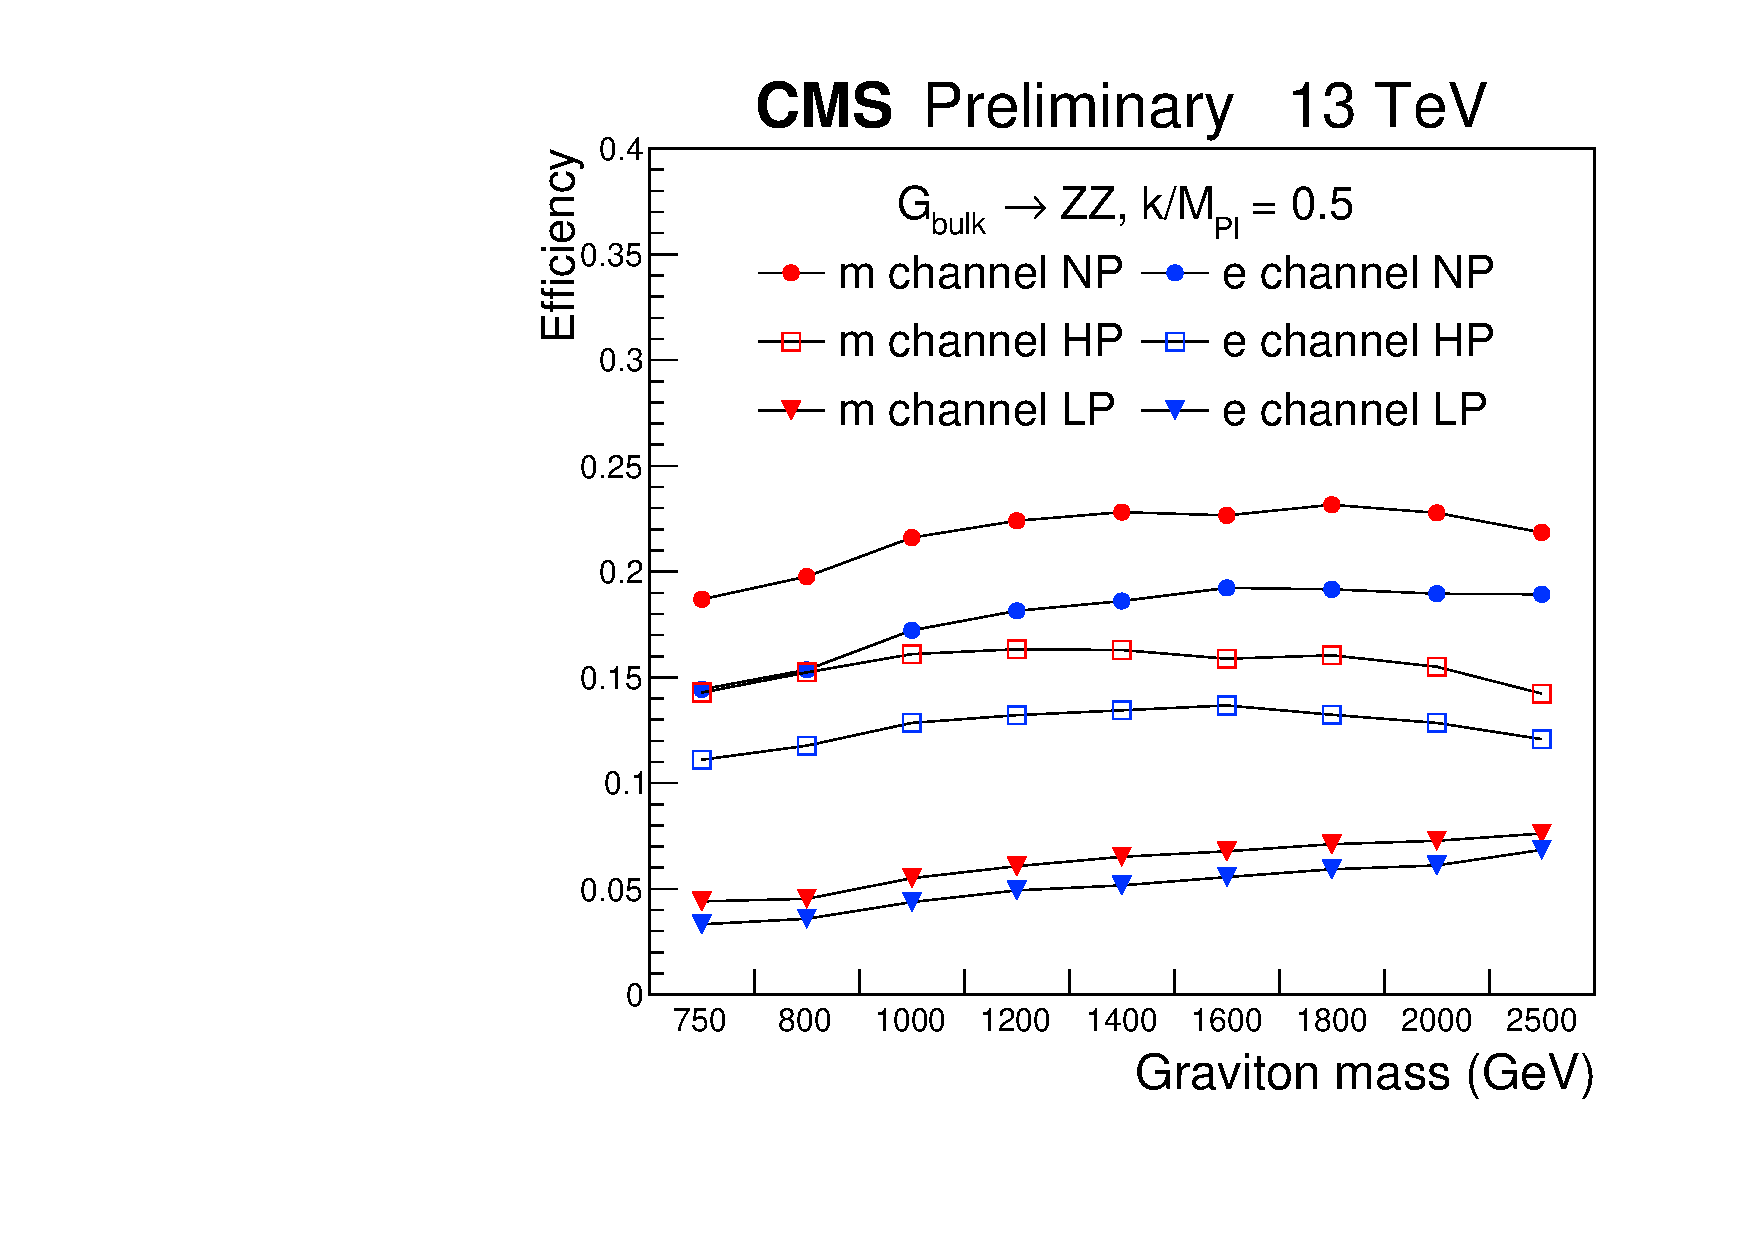
\includegraphics[width=0.60\textwidth]{figures/objects/signalEfficiency.pdf}
\caption[Selection efficiency]{Selection efficiency as function of the bulk graviton mass. Muon (electron) channel is shown with red (blue) markers. The notation in the legend stands for LP=Low Purity, HP=High Purity, and NP=No Purity selection. The denominator entering in the calculation of the efficiencies corresponds to ZZ semileptonic decays into the three lepton flavours.}
\label{selectionEff_VZ}
\end{center}
\end{figure}

A precise description of the analysis cut-flow in the muon and electron channels is provided in the Tables \ref{tab:cutFlowMu} and \ref{tab:cutFlowEl}, respectively. Besides serving as input for the calculation of the signal efficiency, the numbers in the cut-flow tables were important to cross-check the correct performance of the SPRACE analysis framework. The cross-check consisted in a synchronization with other analysis groups, one at the University of Virginia and other at the University of Taiwan. They independently produced identical cut-flow tables using their own analysis frameworks, and the results of the three groups ---Virginia, Taiwan, and SPRACE--- perfectly matched. 

%For a given lepton flavour, the total event selection efficiency is around 75--80\% for muons and 60--70\% for electrons. As we will see, the expected number of background events with high values of invariant mass is practically zero (Fig. \ref{fig:highmass_MVZ}); the maximization of the efficiency is particularly important in that regime.
\begin{landscape}
\begin{table}[p]
%%\footnotesize
%%\scriptsize
\begin{center}
\caption[Cut-flow table muon channel.]{Cut-flow table for different graviton mass points in the muon channel.}
\label{tab:cutFlowMu}
\begin{tabular}{lccccccccc}
\hline
                   &\textbf{M-800} &\textbf{M-1000} &\textbf{M-1200} &\textbf{M-1400} &\textbf{M-1600}  &\textbf{M-1800} &\textbf{M-2000} &\textbf{M-2500} \\ 
 All events        &   50000   &    50000  &    50000  &    49200  &    50000  &    50000  &    48400  &    50000  \\
 Muon events       &   16384   &    16268  &    16402  &    16227  &    16315  &    16534  &    15874  &    16237  \\
 Muon trigger      &   15891   &    15910  &    16084  &    15928  &    15971  &    16141  &    15457  &    15619  \\
 Vertex            &   15891   &    15910  &    16084  &    15928  &    15971  &    16141  &    15457  &    15619  \\
 Muon acceptance   &   15891   &    15910  &    16084  &    15928  &    15971  &    16141  &    15457  &    15619  \\
 Muon ID           &   15876   &    15899  &    16075  &    15920  &    15960  &    16122  &    15440  &    15594  \\
 Dimuon pair       &   14954   &    15176  &    15424  &    15228  &    15284  &    15483  &    14784  &    14824  \\
 Opposite sign     &   14925   &    15156  &    15395  &    15204  &    15257  &    15437  &    14748  &    14779  \\
 Muon isolation    &   14437   &    14689  &    14950  &    14800  &    14834  &    15022  &    14364  &    14397  \\
 Z mass window     &   13667   &    14028  &    14289  &    14155  &    14212  &    14386  &    13773  &    13723  \\
 %Gen. hadronic Z   &   13472   &    13843  &    14105  &    13974  &    14015  &    14170  &    13611  &    13530  \\
 Jet ID            &   13449   &    13836  &    14103  &    13974  &    14014  &    14170  &    13610  &    13530  \\
 Jet Cleaning      &   13373   &    13800  &    14092  &    13970  &    14014  &    14170  &    13610  &    13529  \\
 N-subjettiness    &   12879   &    13549  &    13882  &    13803  &    13863  &    14026  &    13455  &    13367  \\
 Jet Kinematics    &   12366   &    13040  &    13322  &    13227  &    13244  &    13370  &    12812  &    12710  \\
 Invariant mass cut&   12298   &    13012  &    13301  &    13214  &    13233  &    13361  &    12805  &    12705  \\
\hline
\end{tabular}
\end{center}
\end{table}
\end{landscape}

\begin{landscape}
\begin{table}[p]
%%\footnotesize
%%\scriptsize
\begin{center}
\caption[Cut-flow table electron channel.]{Cut-flow table for different graviton mass points in the electron channel.}
\label{tab:cutFlowEl}
\begin{tabular}{lccccccccc}
\hline
	    &\textbf{M-800} &\textbf{M-1000} &\textbf{M-1200} &\textbf{M-1400} &\textbf{M-1600}  &\textbf{M-1800} &\textbf{M-2000} &\textbf{M-2500} \\ 
 All events          &   50000   &    50000  &    50000  &    49200  &    50000  &    50000  &    48400  &    50000 \\ 
 Electron events     &   16484   &    16572  &    16536  &    16094  &    16611  &    16455  &    16037  &    16562 \\ 
 Electron trigger    &   15439   &    15897  &    15996  &    15650  &    16204  &    16063  &    15678  &    16137 \\ 
 Vertex              &   15439   &    15897  &    15996  &    15650  &    16204  &    16063  &    15678  &    16137 \\ 
 Electron acceptance &   15385   &    15853  &    15958  &    15620  &    16167  &    16022  &    15641  &    16077 \\ 
 Electron ID+Iso.    &   15044   &    15433  &    15304  &    14716  &    14987  &    14646  &    14162  &    14575 \\ 
 Dielectron pair     &   11056   &    11694  &    11985  &    12005  &    12425  &    12368  &    12008  &    12355 \\ 
 Opposite sign       &   10880   &    11500  &    11792  &    11801  &    12206  &    12152  &    11793  &    12054 \\ 
 Z mass window       &   10600   &    11240  &    11517  &    11562  &    11954  &    11889  &    11558  &    11805 \\ 
 %Gen. hadronic Z     &   10451   &    11081  &    11370  &    11386  &    11787  &    11733  &    11401  &    11640 \\ 
 Jet ID              &   10428   &    11079  &    11370  &    11386  &    11787  &    11733  &    11401  &    11640 \\ 
 Jet Cleaning        &   10365   &    11066  &    11363  &    11383  &    11786  &    11733  &    11399  &    11640 \\ 
 N-subjettiness      &    9957   &    10839  &    11208  &    11239  &    11641  &    11612  &    11263  &    11498 \\ 
 Jet Kinematics      &    9565   &    10446  &    10809  &    10730  &    11121  &    11087  &    10681  &    10938 \\ 
 Invariant mass cut  &    9536   &    10426  &    10788  &    10723  &    11112  &    11079  &    10672  &    10933 \\ 
\hline
\end{tabular}
\end{center}
\end{table}
\end{landscape}

